%% GABARIT POUR THÈSE PAR ARTICLES
%%
%% Consulter la documentation de la classe ulthese pour une
%% description détaillée de la classe, de ce gabarit et des options
%% disponibles.
%%
%% [Ne pas hésiter à supprimer les commentaires après les avoir lus.]
%%
%% Déclaration de la classe avec le type de grade
%%   [l'un de LLD, DMus, DPsy, DThP, PhD]
%% et les langues les plus courantes. Le français sera la langue par
%% défaut du document. L'option 'bibsection' permet de créer des
%% bibliographies par chapitre présentées sous forme de section
%% numérotée.
% \documentclass[PhD,english,french]{ulthese}
\documentclass[PhD,english,french,nonatbib]{ulthese}
% \documentclass[PhD,bibsection,english,french,nonatbib]{ulthese}
  %% Encodage utilisé pour les caractères accentués dans les fichiers
  %% source du document. Les gabarits sont encodés en UTF-8. Inutile
  %% avec XeLaTeX, qui gère Unicode nativement.
  \ifxetex\else \usepackage[utf8]{inputenc} \fi

  %% Charger ici les autres paquetages nécessaires pour le document.
  %% Quelques exemples; décommenter au besoin.
  %\usepackage{amsmath}       % recommandé pour les mathématiques
  %\usepackage{ncccomma}      % gestion de la virgule dans les nombres
  %% 
  %%\usepackage[toc]{glossaries}      % gestion du glossaire
  %%\makeglossaries

  %% Utilisation d'une autre police de caractères pour le document.
  %% - Sous LaTeX
  %\usepackage{mathpazo}      % texte et mathématiques en Palatino
  %\usepackage{mathptmx}      % texte et mathématiques en Times
  \usepackage[scaled]{helvet}
  \renewcommand\familydefault{\sfdefault} 
  %% - Sous XeLaTeX
  %\setmainfont{TeX Gyre Pagella}      % texte en Pagella (Palatino)
  %\setmathfont{TeX Gyre Pagella Math} % mathématiques en Pagella (Palatino)
  %\setmainfont{TeX Gyre Termes}       % texte en Termes (Times)
  %\setmathfont{TeX Gyre Termes Math}  % mathématiques en Termes (Times)

  %% Packages ajoutés par moi
  \usepackage{todonotes}            % Notes de TODO avec \todo
  \usepackage{multirow}             % Tables avec lignes fusionnées
  \usepackage{alphabeta}            % Lettres grecques hors mode maths
  \usepackage[acronym]{glossaries}  % Glossaire
  \makeglossaries
  \usepackage{appendix}             % Test : Annexes formatées comme voulu
  \usepackage{textgreek}            % Lettres grecques hors formules de maths
  \usepackage{graphicx}             % Affichage d'image
  \usepackage[export]{adjustbox}    % Adaptation d'image à une div
%   \usepackage{listings}
%   \usepackage{xcolor}
  \usepackage{rotating}             % Tourne les figures
  \usepackage{longtable}            % Table sur plusieurs pages
  \usepackage{svg}
  \usepackage{booktabs}             % Tables plus propres avec pre-formatage
  \usepackage{colortbl}             % Couleur dans des tables
  
  \usepackage{titlesec}             % Permet d'utiliser /chapter sans * pour avoir la bonne numérotation
   \titleformat{\chapter}[display]
    {\normalfont\bfseries}{}{0pt}{\Huge}
    
  %% /!\ S'assurer que hyperref est le dernier paquetage chargé.
  \usepackage{hyperref}             % Gestion des hyperliens dans le document
  \hypersetup{colorlinks,allcolors=ULlinkcolor}
  \urlstyle{same}

  %% Redefinition de commande par moi
  
  
  
  
  %% Options de mise en forme du mode français de babel. Consulter la
  %% documentation du paquetage babel pour les options disponibles.https://vpn1.ulaval.ca/+CSCOE+/logon.html
  %% Désactiver (effacer ou mettre en commentaire) si l'option
  %% 'nobabel' est spécifiée au chargement de la classe.
  \frenchbsetup{%
    StandardItemizeEnv=true,       % format standard des listes
    ThinSpaceInFrenchNumbers=true, % espace fine dans les nombres
    og=«, fg=»                     % caractères « et » sont les guillemets
  }

  %% Suppression du numéro de section de la bibliographie. Utilisation
  %% de \extrasfrench parce que c'est la dernière langue déclarée dans
  %% \documentclass, ci-dessus.
%   \addto\extrasfrench{%
  %% Packages ajoutés par moi
  

  %% Déclarations des pages de titre. Remplacer les éléments entre < >.
  %% Supprimer les caractères < >. Couper un long titre ou un long
  %% sous-titre manuellement avec \\.
  \titre{Développement de méthodes et outils d'analyse transcriptomique par réseaux de co-expression de gènes pour la détection de gènes candidats dans le vieillissement humain de différents tissus}
  % \titre{Ceci est un exemple de long titre \\
  %   avec saut de ligne manuel}
  % \soustitre{Sous-titre le cas échéant}
  % \soustitre{Ceci est un exemple de long sous-titre \\
  %   avec saut de ligne manuel}
  \auteur{Gwenaëlle Lemoine}
  \annee{2020}
  \direction{Arnaud Droit, directeur de recherche}
  % \codirection{<Prénom Nom>, <codirecteur ou codirectrice> de recherche}
  % \codirection{<Prénom Nom>, <codirecteur ou codirectrice> de recherche \\
  %              <Prénom Nom>, <codirecteur ou codirectrice> de recherche}

\begin{document}

\frontmatter                    % pages liminaires

\pagestitre                     % production des pages de titre

\chapter*{Résumé}                      % ne pas numéroter
\phantomsection\addcontentsline{toc}{chapter}{Résumé} % inclure dans TdM

\begin{otherlanguage*}{french}
L'analyse par réseau de co-expression de gènes est un outil entré il y a 15 ans dans l'ensemble des outils disponibles pour l'analyse transcriptomique. En étudiant la variation de synchronisation de l'expression des gènes, cet outil permet de révéler de nouveaux gènes impliqués dans des maladies ou phénotypes dont l'expression seule n'est pas significativement différente. Il est également capable de détecter des groupes de gènes, ou modules, interagissant préférentiellement et sur lesquels il est possible d'effectuer une exploration étendue. Il est ainsi possible d'utiliser des méthodes avec injection de connaissance préalable comme l'enrichissement de gènes ou l'association phénotypique, ou des méthodes guidées par les données comme l'analyse topologique ou la co-expression différentielle. Pourtant, ce type d'analyse reste sous exploitée actuellement par rapport à son potentiel, et notamment dans certaines maladies ou phénotypes où l'altération est une désorganisation du système comme le vieillissement. 

Afin de faciliter à tout chercheur l'emploi de cette méthode, un progiciel R disponible sur Bioconductor et nommé GWENA a été développé. Organisé comme un pipeline d'analyse simplifié et allant de la construction du réseau jusqu'à l'aide à l'interprétation des modules entre différentes conditions, c'est également le seul pipeline actuel à intégrer la co-expression différentielle. Pour assister l'utilisateur, il comprend de nombreux avertissements sur l'intégrité des données rentrées et sur la plausibilité des résultats. Afin de limiter le recours à d'autres logiciels, il contient également un système de visualisation des réseaux. Enfin, GWENA est un outil dont l'architecture modulaire lui permettra d'évoluer avec le temps.

L'efficacité de GWENA a été démontrée dans une première étude du vieillissement du muscle squelettique humain où un sous ensemble de gènes a été priorisé pour l'étude de la sarcopénie. Il a également permis de préciser une topologie du réseau spécifique du vieillissement et observée auparavant : la perte de connectivité du réseau, ou déconnexion. En effet, parallèlement à la déconnexion, il a été constaté grâce à GWENA une reconnexion locale située au niveau des gènes pivots. Pour étudier cette topologie à large échelle, l'analyse a été répétée sur un ensemble élargi de tissus humains. Par un recoupement des modules différentiellement exprimés, des phénomènes communs du vieillissement entre tissus sont apparus ainsi que des phénomènes spécifiques à certains tissus. L'analyse topologique, notamment de la déconnexion, des gènes inclus dans ces recoupements pour deux exemples, un phénomène commun et un phénomène spécifique, a à son tour permis la priorisation de gènes encore mal étudiés ou inconnus dans ces phénomènes.

En finalité, les travaux présentés au cours de cette thèse auront amené à la création d'un outil utile à la communauté de biologistes comme bio-informaticiens pour faciliter l'accès à une analyse à a haut potentiel dans l'analyse du vieillissement et toute autre condition, notamment celles axées sur la dérégulation de l'expression systémique.

\textbf{Mots-clefs :} co-expression, réseau, vieillissement, transcriptomique, progiciel R, Bioconductor, co-expression différentielle.
\end{otherlanguage*}
                % résumé français
\chapter*{Abstract}                      % ne pas numéroter
\phantomsection\addcontentsline{toc}{chapter}{Abstract} % inclure dans TdM

\begin{otherlanguage*}{english}
  Text of English abstract.
\end{otherlanguage*}
              % résumé anglais
\cleardoublepage

\tableofcontents                % production de la TdM
\cleardoublepage

\listoftables                   % production de la liste des tableaux
\cleardoublepage

\listoffigures                  % production de la liste des figures
\cleardoublepage

\chapter*{Acronymes}                      % ne pas numéroter
\phantomsection\addcontentsline{toc}{chapter}{Acronymes} % inclure dans TdM              % acronymes

\dedicace{Dédicace si désiré}
\cleardoublepage

\epigraphe{Texte de l'épigraphe}{Source ou auteur}
\cleardoublepage

\chapter*{Remerciements}         % ne pas numéroter
\phantomsection\addcontentsline{toc}{chapter}{Remerciements} % inclure dans TdM

Je remercie mon directeur, le Dr. Arnaud Droit, pour m'avoir accueillie dans son laboratoire.

Merci également aux membres du jury, la Dre. Francine Durocher, le Dr. Simon Hardy, le Dr. Yoann Bossé, la Dre. Sarah Gagliano Taliun, pour avoir accepté de siéger et évaluer mes travaux.

Enfin, merci à tous mes proches qui m'ont accompagnée durant ces années.
         % remerciements
\chapter*{Avant-propos}         % ne pas numéroter
\phantomsection\addcontentsline{toc}{chapter}{Avant-propos} % inclure dans TdM

% L’avant-propos contient les renseignements sur:
% - l’état de publication des articles intégrés (dates de soumission, d'acceptation ou de publication)
% - les modifications entre la version intégrée de l’article et sa version publiée, s’il y a lieu 
% - votre statut d’auteur (principal ou non)
% - votre rôle exact dans la préparation de chaque article
% - les coauteurs de chaque article

\section{Projets principaux}

Cette thèse est réalisée avec l'insertion d’articles écrits durant mon doctorat. Elle présente l’état de mes travaux dont le but principal était le développement d’outils et méthodes pour la détection de gènes candidats au vieillissement humain par l'utilisation de réseaux de co-expression de gènes. Chaque chapitre est donc constitué d'un article publié ou visant à l'être.

Les articles insérés sont les suivants :
\begin{itemize}
    \item \textit{GWENA: gene co-expression networks analysis and extended modules characterization in a single Bioconductor package}, publié dans la revue \textit{BMC Bioinformatics} le 25 mai 2021.
    \item \textit{Analyse trans-tissus par réseau de co-expression de gènes pour la détection de fonctions physiologiques communes et spécifiques au vieillissement}, article à traduire et soumettre dans la revue PLoS One.
\end{itemize}


\section{Contribution à l'article "GWENA"}

Je suis responsable de la conception, développement et maintenance de l'outil GWENA ainsi que de l'écriture de l'article. D'un point de vue analyse pour le cas d'utilisation, je suis responsable du traitement des données ainsi que de leur analyse. Le choix de la méthodologie fut un travail conjoint de Marie Pier Scott-Boyer qui a également supervisé le projet. Elle a également avec Olivier Périn, Bathilde Ambroise et Arnaud Droit participé à la relecture de l'article. L'intégralité de l'article a été validé par tous les auteurs. Arnaud Droit s'est également chargé de la recherche de financement.


\section{Contribution à l'article d'analyse trans-tissus du vieillissement via GWENA}

Je suis responsable de la conception du projet, du traitement et de l'analyse des données, de l'interprétation des résultats, et de la rédaction de l'article. Marie Pier Scott-Boyer a assisté dans la consolidation de la méthodologie et sa validation. Arnaud Droit s'est chargé de la recherche de financement.


\section{Projets annexes}

Durant mon doctorat, j'ai également pu m'investir dans différents projets scientifiques :
\begin{itemize}
    \item \textit{Weighted gene co-expression network analysis identifies inflammaging biomarkers in aged skin of humans in vivo}. Projet de ré-analyse des données de transcriptomique de Kuehne et al. 2017 par le biais de GWENA. Il a permis de mettre en évidence des gènes impliqués dans le phénomène d'inflammation chronique de faible intensité dans des biopsies d'épiderme. Par respect envers la clause de confidentialité de la chaire de recherche et d'innovation L'Oréal en biologie numérique, ces travaux n'ont pas été soumis à publication.
    \item Étude à travers de multiples points temporels sur 28 jours de la reconstruction épidermique basée sur un modèle d'épiderme \textit{in vitro} provenant de biopsies de circoncisions. Travaux effectués pour la chaire de recherche et d'innovation L'Oréal en biologie numérique et confidentiels.
\end{itemize}


\todo[inline]{Si projets non doctoraux ajoutés en annexe (ACCEM, illustration scientifique, bioinfo-fr.net, mette cette phrase : D'autre travaux scientifiques non académiques ont également été réalisés et sont visibles en Annexe \\ref{}}


\section{Financements}

Les travaux présentés dans cette thèse ont étés soutenus par la Chaire de recherche et d'innovation L'Oréal en biologie numérique.

\section{Notes}

\begin{itemize}
    \item L'intégralité des figures a été réalisée par mes soins et est sous licence CC-BY-NC sauf mention contraire ou citation d'une figure d'une publication.
    \item L'article situé en Chapitre \ref{chapter:gwena} est publié dans BMC Bioinformatics sous la licence CC-BY
    \item Pour plus d'information sur les licences Creative Commons : \url{https://creativecommons.org/about/cclicenses/}
\end{itemize}           % avant-propos

\mainmatter                     % corps du document

%%%%%%%%%%%%%%%%%%
%% INTRODUCTION %%
%%%%%%%%%%%%%%%%%%

\setcounter{chapter}{1}         % permet de débuter l'intro à 1. au lieu de 0.
\chapter*{Introduction}         % enlève la numérotation
\phantomsection\addcontentsline{toc}{chapter}{Introduction} % inclus l'intro dans la table des matières
\graphicspath{ {./img/intro} }

%% ######################
%% GROSSE AIDE A LA BIBLIO https://www.connectedpapers.com
%% #####################




%%%%%%%%%%%%%%%%%% LA COMPLEXITÉ DU VIVANT %%%%%%%%%%%%%%%%%%

\section{La complexité du vivant}

\subsection{D'un code unique à un fonctionnement multiple}

Bien que toutes les cellules d'un organisme possèdent la même information génétique via un ADN identique, plusieurs types cellulaires de fonction différente cohabitent pour former des tissus variés. Ces différences provennant d'un contrôle de l'expression ou de la répréssion d'un gène sont le fruit d'un ensemble de mécanismes de régulation établis dès les premières différenciations cellulaire dans le développement d'un organisme. Différentes types de mécanismes vont alors impacter la qualité et la quantité d'ARN messager (ARNm) produit par les cellules :
\begin{itemize}
\item La régulation de l'initiation de la transcription : la fixation d'une protéine sur l'ADN entraine l'impossibilité de fixation de l'ARN polymérase ou à l'inverse favorise son recrutement pour la transcription d'un gène.
\item  La conformation de la chromatine : les repliements de l'ADN pour la condenser dans une cellule implique de rendre disponible certaines régions à la transcription et indisponible d'autres.
\item La modification post transciptionnelle : les ARNm nécessitent l'ajout d'une 7-methylguanosine sur l'extrémité 5' (coiffe 5'), un épissage alternatif, et une polyadenylation (queue poly A) sur l'extrémité 3' afin d'être traduits en protéine. En leur absence, ces ARNm sont détruits par la cellule.
\item  La méthylation : les îlots CpG situés sur l'ADN (notamment dans les promoteurs) peuvent subir l'ajout d'un groupement méthyl, empêchant alors la fixation de différents agents de la transcription.
\item La susceptibilité à la dégradation : afin de perdurer plus de quelques minutes dans la cellule [\^Yu\_2001], certains ARN contiennent ou évitent certains motifs de nucléotides (éléments riches en AU, codon stop prématuré, taille de queue poly-A) ou bien sont victimes d'ARN non codants (ARNmi et ARNip) qui vont favoriser leur dégradation
% \item [^Yu_2001]: Yu J, Russell JE. Structural and functional analysis of an mRNP complex that mediates the high stability of human beta-globin mRNA. Mol Cell Biol. 2001;21(17):5879-5888. doi:10.1128/mcb.21.17.5879-5888.2001 
\item La régulation de la traduction : le contrôle du recrutement des sous unités des ribosomes, leur altération, ou la compétition des ARN de transfert (ARNt) pour la terminaison sont des paramètres impactant la production finale d'une protéine sans erreur et ne sera donc pas dégradée.
\end{itemize}


Lors des perturbation (maladie, stress, âge, etc.) du fonctionnement cellulaire normal, sain, cette régulation de l'expression s'en retrouve pertubée. Le transcriptome (ensemble des ARN ou transcrits produits) est alors un témoin direct des fonctions mises en défaut. L'étude de la quantité de chacun donne ainsi un moyen direct direct de comprendre l'origine d'effets macroscopiques (irritation atopique, tumeur, nécrose, etc.) ou moléculaires (augmentation du taux de glucose, malabsorption de nutriments, augmentation du pH, etc.).

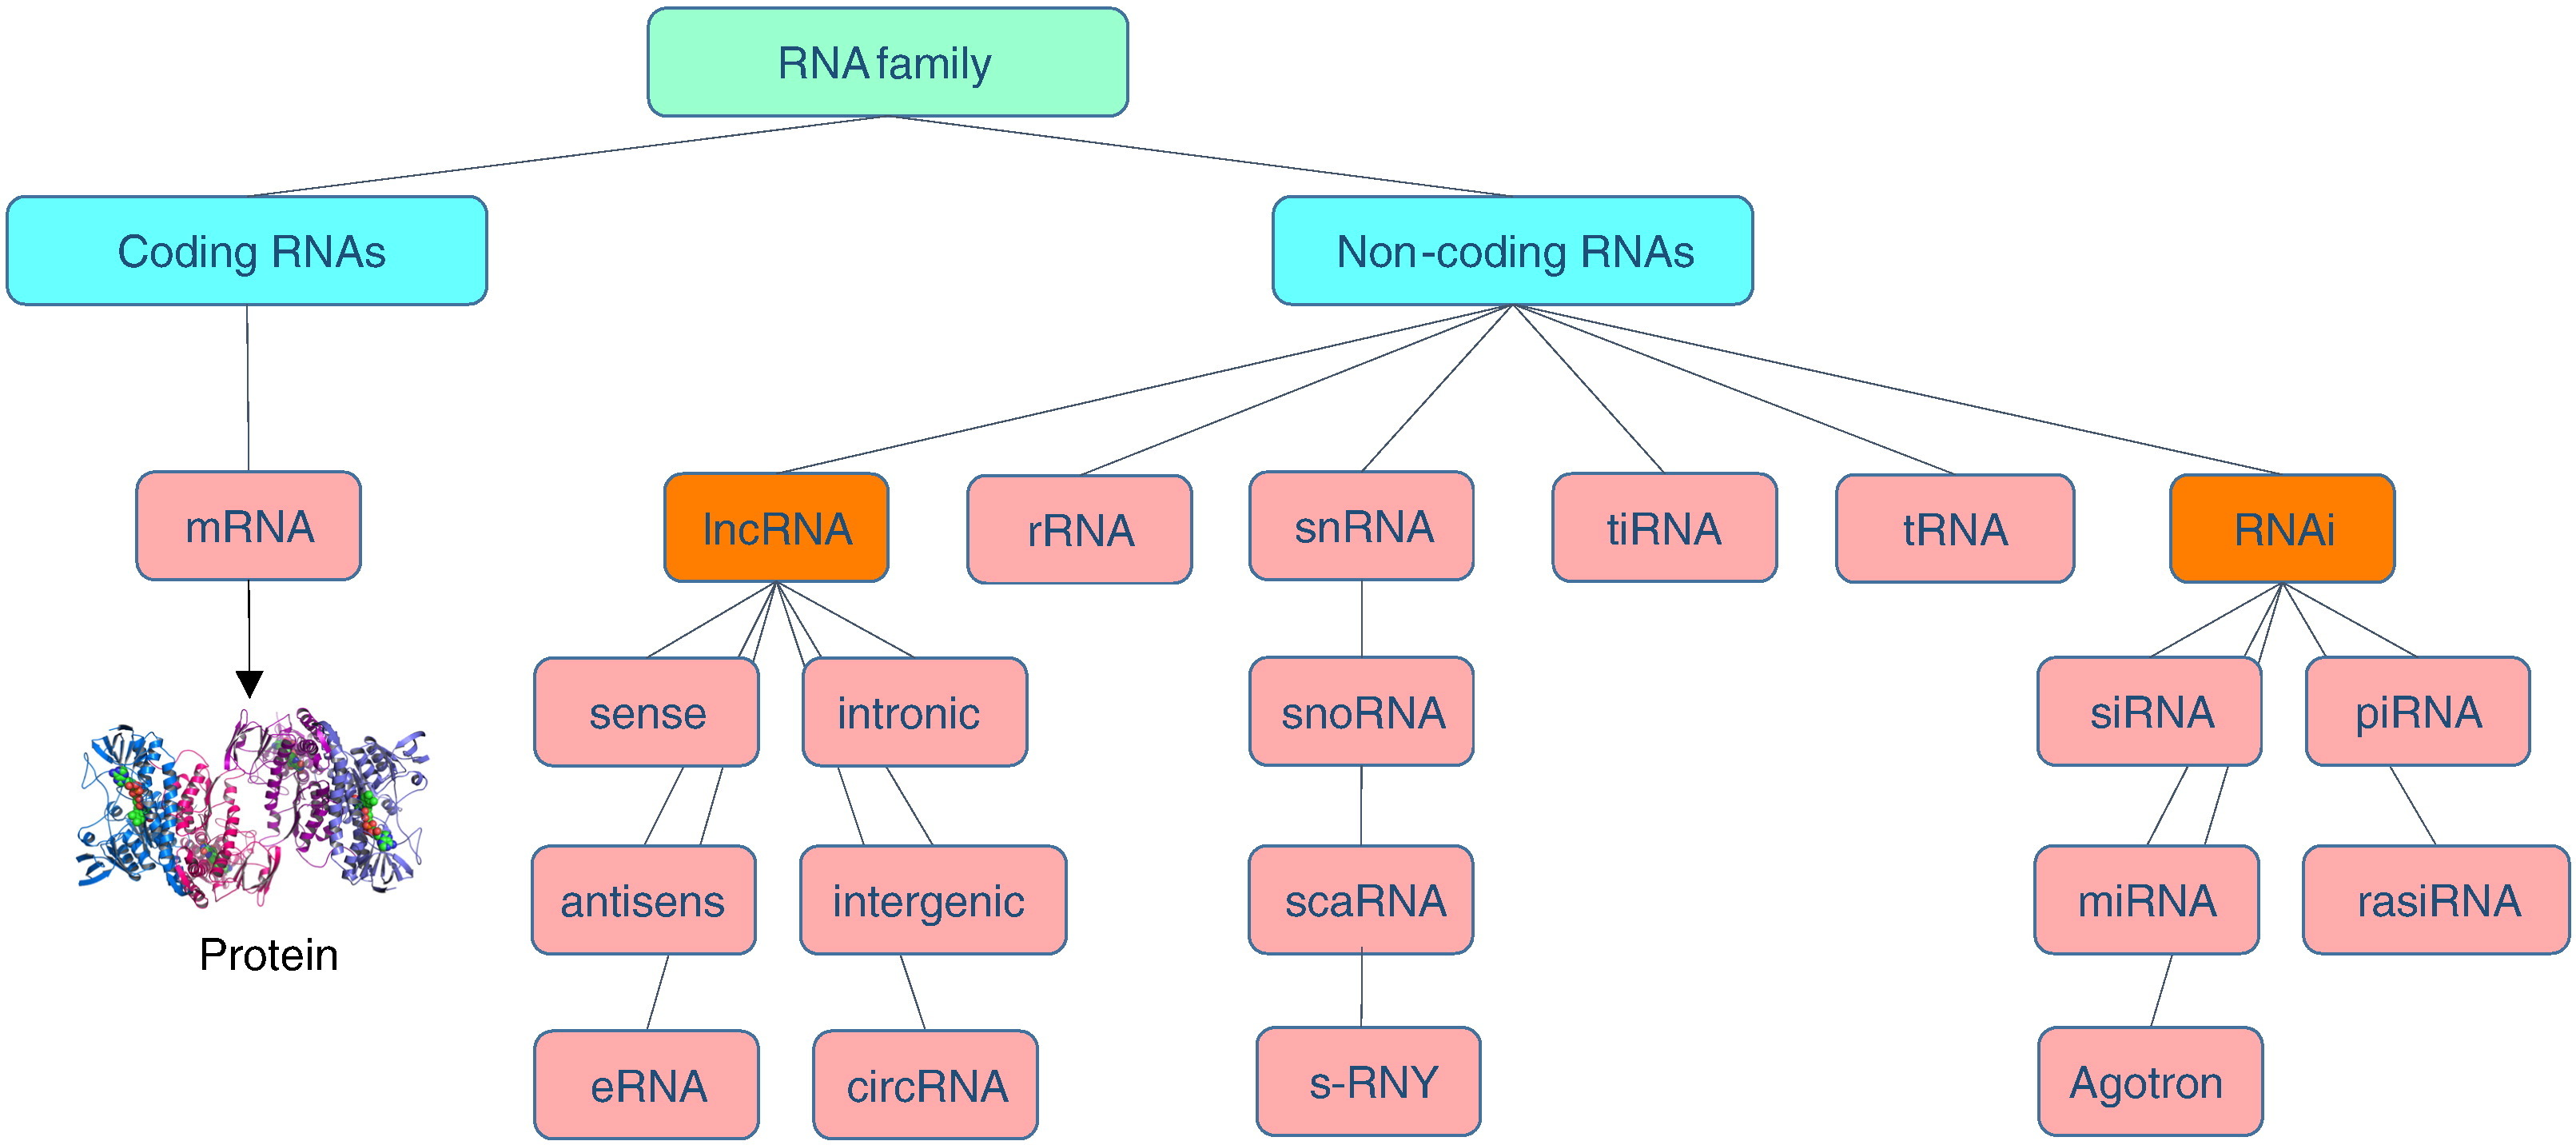
\includegraphics{img/intro/rna_familly_tree.jpg}

%% TRANSITION : parler des erreurs/variabilité biologique ? 

% \subsection{L'étude des perturbation du vivant pour la résolution de conditions cliniques}
\subsection{L'étude des perturbation de l'expression pour la résolution de conditions cliniques}

\section{Les technologies de séquençage de l'expression des gènes}
%% TODO : merge avec 1.1 partie d'avant

%% Nb publi pour le ration de microarray / RNA seq de jeux de données ?


%% historique des techno et qques specificités : https://journals.plos.org/ploscompbiol/article?id=10.1371/journal.pcbi.1005457
\begin{itemize}
\item Avant propos sur le développement des technologies de séquençage avec la quantification d'ARNm par rt-qPCR, le séquençage par gel, etc.
\item Transition vers les technologies de séquençage nouvelle génération
\end{itemize}

%% Un TRES bon site sur les technos de sequencage : http://education.knoweng.org/sequenceng/

\subsection{Microarray}
\begin{itemize}
\item Principe
\item Utilisation avec des exemple
\item Propriétés mathématiques et techniques
\begin{itemize}
    \item Distribution
    "Données continues, il est possible de construire des modèles d’analyse statistique ense basant sur des hypothèses de normalité des données (Smyth, 2004). Ces techniquesd’analyse, adaptées aux données gaussiennes ne peuvent pas être appliquées directementaux données RNA-seq qui sont des données de comptage, discrètes et positives" %% https://tel.archives-ouvertes.fr/tel-01424124/document
    \item Normalisation : Normalization is a process designed to identify and correct
technical biases. 2 types of norm : Between and within normalization (cf. formation marie laure meme si c'est pour le RNA-seq). Pourquoi normalisation log2 : le log pour passer à une échelle symétrique autour de 0, le 2 car c'est + facile à interpréter, chaque fois qu'on augmente le ratio Ti de 1, on double la up regulation  %%(https://www.researchgate.net/post/Why_do_we_usually_use_Log2_when_normalizing_the_expression_of_genes et https://www.nature.com/articles/ng1032z)
    \item Contrôle qualité
    \item Filtration
\end{itemize}
\item Explication du déclin mais avec contraste sur son utilité quand pas besoin de whole transcriptome
\end{itemize}

\subsection{RNA-Seq}
\begin{itemize}
\item Principe
\item Un mot sur le fait qu'on applique pas les mêmes méthodes de normalisation car la nature du signal n'est pas le même : une fluorescence pour le microarray (variable continue), et un comptage dans le cas du RNA-seq (variable discrète).
\item Explication de l'essor du RNA-seq (couts, precision, etc.)
\item Propriétés mathématiques : distribution(binomiale negative) %% Justification binomiale negative "Negative binomial (NB) distribution is the established gold standard, because of its ability to accurately model RNA-seq data with a low number of available replicates [7]." https://doi.org/10.1093/bib/bbx115
\item normalisations : %% cf. formation marie laure, il y a toutes les refs de publi a prendre
%% La raison du l'utilisation des pseudo counts et du log dans le RNA-seqyo : https://www.biorxiv.org/content/biorxiv/early/2020/05/19/2020.05.19.100214.full.pdf
\begin{itemize}
    \item Within sample
    \item Between samples
\end{itemize}
%% À classer entre within/between plus ahut selon ce qui est marqué dans la formation de marie laure : taille de librairie (= profondeur de sequencage), contenu en GC, taille des gènes, composition de la population d'ARN de chaque condition), contrôle qualité, filtration  (https://www.biostars.org/p/349881/)
\end{itemize}


%%%%%%%%%%%%%% LE TRAITEMENT STATISTIQUE DE L'INFORMATION BIOLOGIQUE %%%%%%%%%%%%%%


\section{Le traitement statistique de l'information biologique}
\subsection{L'expression différentielle : les acteurs majeurs}
\begin{itemize}
  \item Méthode de capture des acteurs majeurs
  \item Pas d'étude du système 
% \item Des statistiques descriptives à l'expression différentielle %% Bof, j'ai pas retrouvé de stade "stats explo" 
\end{itemize}

\subsection{La modélisation du vivant : des acteurs au système}
\begin{itemize}
\item De la régulation des gènes à son approximation par des modèles statistiques, en passant par la biologie des systemes qui est trop couteuse pour des organismes complexes %% mal formulé car dans le desordre (le dernier point devrait venir en 2e)
\item Transistion vers la modélisation par encodage de l'information dans des réseaux qui sont en fait des graph et qui sont moins couteux car probabilistes (ils ne sont pas la vérité mais une approximation)
\end{itemize}

\subsection{Les réseaux biologiques : le système vu via la théorie des graphes}
\begin{itemize}
\item Principe : les graphes sont une méthode de plus en plus utilisée dans la représentation du fonctionnement d'organismes puisqu'ils permettent d'avoir une vision à l'échelle du système tout entier.
%% Jolie intro à s'inspire : https://www.nature.com/articles/s41467-019-08746-5
\item Différences / ressemblance entre graphe et reseau ?
\item Les types de réseaux/graphes rencontrés en biologie et plus particulièrement en expression des gènes : small-world
\item Les problèmes de visualisation de grands réseaux %% section layout de ce livre https://sites.fas.harvard.edu/~airoldi/pub/books/BookDraft-CsardiNepuszAiroldi2016.pdf
\end{itemize}


%%%%%%%%%%%%%%%%%% LES RESEAUX DE CO-EXPRESSION %%%%%%%%%%%%%%%%%%


\section{Les réseaux de  co-expression}

%% GROOOOOSSSE PUBLI REVIEW sur la co-expression ET la comparaison de modules, aka co-expr differentielle https://doi.org/10.1109/TCBB.2019.2893170

\subsection{But}
"Gene co-expression networks seek to identify transcrip- tional patterns indicative of functional interactions and regulatory relationships between genes" %%https://genomebiology.biomedcentral.com/articles/10.1186/s13059-019-1700-9 + Barabási A-L, Gulbahce N, Loscalzo J. Network medicine: a network-based approach to human disease. Nat Rev Genet. 2011;12:56–68. + Furlong LI. Human diseases through the lens of network biology. Trends Genet. 2013;29:150–9.

\subsection{Principe}
%% Relire `van Dam, S., Võsa, U., van der Graaf, A., Franke, L. & de Magalhães, J. P. Gene co-expression analysis for functional classification and gene–disease predictions. Brief. Bioinform. bbw139 (2017). doi:10.1093/bib/bbw139`
\begin{itemize}
    \item Réseaux binaires (0 = pas de connexion, 1 = connexion). Pour et contres.
    \item Réseaux pondérés. Pourquoi c'est vers ça qu'on s'est orientés ? Car les connections entre gènes ne sont pas binaires, elles sont plutot multiples et très dépendantes temporellement. Une meme cellule échantillonnée à des temps différents aura un profil plus ou moins différent. On y retrouvera les grandes fonctions clefs mais les aspects plus variables auront peut etre changé. D'où aussi la nécessité d'un bon nombre d'échantillons pour assurer la validité des résultats. Sinon les correlations ne sont pas représentatives.
\end{itemize}
\subsection{Construction}
\begin{itemize}
\item Les différents scores de similarité : Pearson, Spearman, bicor, mutual information
\item La pondération des scores (adjacence et TOM) et la propriété d'invariance d'échelle (scale-free). Reparler de barbarasi et son celebre article (https://science.sciencemag.org/content/325/5939/412/tab-pdf) + Pourquoi elle est parfois encore discutée (https://www.nature.com/articles/s41467-019-08746-5) alors que tout de même pertinente en biologie. 
\end{itemize}
\subsection{Détection de modules}
\begin{itemize}
    \item Notion de communauté
    \item Définition du partitionnement (clustering) et des différentes techniques
\end{itemize}

\subsection{Exploitation des modules de gènes}

\subsubsection{Intégration biologique}
%% AKA knowledge driven
\begin{itemize}
    \item Enrichissement
    \item Test d'association
\end{itemize}

\subsubsection{Association phenotypique}
%% aussi knowledge driven

%%\subsection{Capitalisation sur l'information intrinsèque aux données}

\subsubsection{Étude topologique}
%% AKA data driven

%% Note : à voir si je présente aussi ici la comparaison de module vu que je vais ptet évoquer l'expression differentielle ici pour faire le parallele avec l'analyse transcripto classique. Sinon ça ira dans l'intro du chapitre avec l'article de GWENA.

\begin{itemize}
    \item Degré
    \item Définition de hub gene
    A trier / ordonner entre les différentes définitions, ce qu'elles visent, ce qu'elles appaortent et si possible une comparaison d'entre elles. On distinguera les mesure purement basées sur la theorie des graphs et celles impliquant des mesures statistique de significativité d'un gene comme hub (cf publi sur DHGA)
    \begin{itemize}
        \item Def 1 : Network theory : "A node is defined as hub node, if its connection degree is greater than average connection degree of the network" %% https://www.ncbi.nlm.nih.gov/pmc/articles/PMC5215982/
        \item Def 2 : Network hubs, the core elements in the network, can be defined using a range of different measures. These measures quantify distinct aspects of topological centrality, which can be defined as the capacity of a node to influence or be influenced by other nodes by virtue of its connection topology (Fornito et al., 2016).
    \end{itemize}
\end{itemize}
\subsubsection{Expression différentielle}
Pas sur de foutre ca là... Peut etre plutot en intro de la section complete en guise de "En analyse RNA classique, une méthode data driven est l'expression différentielle, mais en co-expression on a a disposition plus d'information extractable, et ce grace a la theorie des graphes" 

\subsubsection{Comparaison de modules}

Ou co-expression différentielle
%% "However, searching for differences in networks requires great sensitivity to the initial choice of data. For example, the absence of a shared link in mouse and human co-expression networks does not necessarily indicate divergent function. Instead, differences in the mouse and human co-expression networks may indicate differences in the technical platforms or the experimental conditions used to build the networks" http://doi.org/10.1371/journal.pgen.1000776

\subsection{Interprétation des résultats}

\subsubsection{Comparabilité des résultats issus de RNA-seq et de microarray}
\begin{itemize}
    \item Pas les meme hub genes %% "Microarray and RNA-seq-derived networks have different hub genes" https://academic.oup.com/bioinformatics/article/31/13/2123/196230
\end{itemize}


%%%%%%% L'INTÉRÊT DE l'ANALYSE PAR CO-EXPRESSION POUR L'ÉTUDE DU VIEILLISSEMENT %%%%%%%


\section{Le vieillissement, système hautement imbriqué}
%% Idée de début de paragraphe
S'il est une condition biologique où les réseaux de co-expression sont particulièrement bien adpatés, c'est bien le vieillissement. Source multi-factorielle de changements dans l'organisme, il est chez l'humain à l'origine d'une dégradation progressive des fonctions de base du corps.

\subsection{Définition biologique}
\begin{itemize}
    \item Facteurs : raccourcissement des télomères, phénomènes d'inflammation, réduction de la machinerie cellulaire
    \item Manifestation : Ralentissement de la division cellulaire, développement de cellules non-fonctionnelles / nocives (aka tumeurs), malfonctionnement des tissus/organes
\end{itemize}

\subsection{Enjeux}
Un enjeu de santé publique
\begin{itemize}
    \item Susceptibilité aux maladies opportunistes
    \item tdeetAutonomie patient
    \item Médicalisation précoce
\end{itemize}

\subsection{La capture de l'information liée au vieillissement par la transcriptomique}

\begin{itemize}
    \item La dérégulation de la transcription comme phénomène précédemment mentionné
    \item L'insuffisance de la capture de biomarqueurs pour un processus aussi compliqué que le vieillissement. Donc la nécessité d'une étude en réseau
    \item 
    
\end{itemize}
%% https://doi.org/10.1007/978-981-32-9005-1_3


\section*{Phrases utiles à retravailler et intégrer}

\begin{itemize}
\item "Studies have shown that each gene is estimated on average to interact with four to eight other genes1 and to be involved in 10 biological functions" [10.1038/s41598-017-18705-z]
\item "A very clear partition of different biological networks is provided by Christensen et al. [1], who separated these networks into five main categories as follows: [metabolic networks, signal transduction networks,transcriptional regulatory networks, protein-protein networks, functional gene networks]" [10.1093/bfgp/elt003]
%% Bouquin à la coloc de Clément à Sète, pas retrouvé sur le net jusque là 
\item "Le vieillissement est un continuum conduisant une personne en bonne santé à une réduction de sa réserve fonctionnelle, puis de sa capacité fonctionnelle et de sa qualité de vie. CEs différents aspects ne décrivent pas un chemin linéaire ou ordonné." [Patient agé : particularités de la consultation, Gilles Berrut]
\item "It has been reported that nearly one in four studies uses public data to address a biological problem without generating new raw data (Rung and Brazma, 2013)." [10.3389/fpls.2016.00444]
\end{itemize}


%% Points que je veux aborder :
%%  - Definition des reseau arrete / noeud
%%  - Definition des modules par l'effet de modularité
%%  - Ce à quoi ils peuvent servir : raccrochage de fonction a certains genes, detection de pathways, detection de reseaux de regulation



%%    • Weighted aspect [trop general, aura plutot sa place dans la thèse]
%% But because of the multi-functionality aspect of each gene, such GCN using only binary state between genes (1 = correlated, 0 = not correlated) lead to information loss\cite{Langfelder2008}. Therefore, a new class of GCN have been developed: weighted gene co-expression networks. One of the most famous implementation is the R package WGCNA\cite{Langfelder2008}, but one can also mention the recent wTO\cite{Gysi2018} package which consider both positive and negative correlation for GCN building. Instead of a simple pairwise correlation, these packages weight the similarity score by calculating a factor taking into account other properties of the network. In the case of WGCNA, it specifies an adjacency score which raise the similarity to a power, which will increase the strength of strong similarities while keeping low week ones. In the case of wTO, it determine an average accounting for all common neighbors of a node.

%%    • Topological aspect
%%    • Co-expression properties (Scale-free-network entre autres ?)



%% Infos sur la peau : these super interessante => https://dumas.ccsd.cnrs.fr/dumas-01599807/document% \end{itemize}

          % introduction
\chapter{Titre du chapitre}     % numéroté

Texte du chapitre.



%% \bibliographystyle{unsrt}     % style de la bibliographie
%% \bibliography{}               % production de la bibliographie    % chapitre 1
\setcounter{chapter}{3}
\chapter*{Chapitre 2 - À définir}
\phantomsection\addcontentsline{toc}{chapter}{Chapitre 2 - À définir} 
%%\chapter{Titre du chapitre}     % numéroté

Idées :
\begin{itemize}
    \item Rajout d'information protéique pour "consolider" le réseau ?
    \item Rajout d'une méthode de réseau consensus à GWENA ?
    \item ???
\end{itemize}

\section{test bis}

\bibliographystyle{}              % style de la bibliographie
\bibliography{}                   % production de la bibliographie
    % chapitre 2, etc.
\chapter*{Conclusion}         % ne pas numéroter
\phantomsection\addcontentsline{toc}{chapter}{Conclusion} % dans TdM

Une thèse ou un mémoire devrait normalement se terminer par une
conclusion, placée avant les annexes, le cas échéant. Celle-ci est
traitée comme un chapitre normal, sauf qu'elle n'est pas numérotée.


% Publi utile pour les perspectives :
% https://onlinelibrary.wiley.com/doi/abs/10.1111/gbb.12106


Le vieillissement est un phénomène dont la complexité n'a d'égal que la multiplicité de ses manifestations. Tantôt origine, tantôt conséquence, les phénomènes de sa manifestations impactent de nombreux mécanismes cellulaire et moléculaires : sénescence et cellules souches, inflammation chronique de faible intensité, raccourcissement des télomères, etc. \cite{Lopez-Otin2013}. Pour distinguer de façon certaine chacun des altérations basales chez chaque individu, un nombre important d'échantillons est nécessaire. L'étude GTEx est à ce jour le plus gros regroupement de séquençage en terme d'individus/tissus non ciblé sur une pathologie. Sa réalisation permet d'étudier le vieillissement non plus dans ses manifestations les plus détaillées mais bien de rechercher les mécanismes communs à beaucoup des tissus composant le corps humain. Cependant            % conclusion
\setcounter{chapter}{5}
\setcounter{section}{0}
\setcounter{figure}{0}   
\chapter*{Discussion}         % ne pas numéroter
\phantomsection\addcontentsline{toc}{chapter}{Discussion} % dans TdM

\section{L'apport de mes travaux sur l'étude du vieillissement}

\begin{itemize}
    \item La création d'un outil de type pipeline avec comparison et analyse intégrée
    \item La démonstration de son application chez le muscle et le ciblage de gènes potentiellements liés au vieillissement
    \item whatever secodn article
    \item Les études de quantification de l'expression c'est bien, mais grâce au RNA-seq on peut aller explorer d'autres pan du transcriptome et potentiellement faire des recoupements avec des phénomènes/mécanismes observés via quantification de l'expression
\end{itemize}

\section{limitations}
\begin{itemize}
    \item Les réseaux de co-expression comme moyen d'étude mais de nouvelles méthodes moins bruitée se mettent en place %% https://www.nature.com/articles/s42255-020-00304-4 et https://www.nature.com/articles/s42255-020-00295-2 (pas un article mais un News and Views qui resume)
    \item Ne permettent pas directement de connaitre le sens de régulation, il faut d'autres analyses pour inférer le sens de la relation dans un réseau de co-expression. Avec ça vient les soucis d'inférence évoqués par marie laure : co-regulation, manque de puissance stat..
\end{itemize}



\section{Perspectives}

- la potentielle application dans l'étude du cancer ou dans une étude comparative concernant la perte de connectivité observée là bas également 10.1371/journal.pone.0087075
- l'utilisation dans des populations d'ethinies plus minoritaires, malheureusement les données et bdd sont faibles par rapport à la puissance stat requise
- approches multi-omiques avec intégration de réseaux protein-protein % <- ptet plus dans mise en contexte des travaux            % discussion


\bibliographystyle{plain-fr}    % bibliographie
\bibliography{bibliographie}    % nom du fichier .bib

% \appendix                       % annexes le cas échéant
% \chapter*{Annexes}
% \addcontentsline{toc}{chapter}{Annexes}
% \chapter{Questions en bio-informatique}

Cette annexe a pour vocation de regrouper les nombreuses questions qui ont pu se poser durant cette thèse. Bien que parfois basiques, elles n'en sont pas moins légitimes. Beaucoup de ces questions on vu leur réponse plus longue que prévu à trouver en raison de consensus installés dans la communauté, de reflex de chercheur, etc. sans savoir l'origine de ceux-ci.

\section{Pourquoi normalisation log2 pour le microarray ?}
Le log pour passer à une échelle symétrique autour de 0, le 2 car c'est + facile à interpréter, chaque fois qu'on augmente le ratio Ti de 1, on double la up regulation 
%% (https://www.researchgate.net/post/Why_do_we_usually_use_Log2_when_normalizing_the_expression_of_genes et https://www.nature.com/articles/ng1032z)

      % annexe
% \chapter{NetRep statistics detail}


\todo{TODO : récupérer, résumer (et traduire ?) l'explication et l'interprétation biologique des 7 métriques disponibles dans les Supplemental Experimental Procedures de la publication de netrep (https://doi.org/10.1016/j.cels.2016.06.012)}

Source : Document S1. Supplemental Experimental Procedures, Figures S1–S7, and Tables S1–S4, S6, and S7 from 

% \chapter{Demande d'accès dbGaP aux données protégées de GTEx}

\label{annexe:dbgap}

\section{Query title}
Muscle gene co-expression in multiple age range for sarcopenia condition exploration

\section{Research use statement}
As a multi factorial phenomena, aging is a complex condition to study. Current analysis of transcriptomic data joined with phenotypic ones have unravel few genes and environmental variables impacting it. However, aging remains not fully understood. These may come from current approaches focusing on single factors while aging is more about interaction between many of them. This is why we would like to study it through the spectrum of the co-expression networks. However, because aging is already complex by itself, we will focus on a single tissue in the beginning : muscle. Reasons are myopenia and dynapenia (known together as sarcopenia) are responsible for loss of autonomy, weak metabolic aggression resistance, and increased mortality.
By using our yet to be published pipeline developed in our lab, we aim to build gene co-expression modules and network from transcriptomic data and characterize them with external resources. This pipeline begin with a quality assessment of the data, based on the technique used to get transcriptomic information (either microarray or RNA-Seq). It then compute co-expression levels and detects modules by using the WGCNA package. Additionnal steps are then performed to fully charachterize the modules : biological enrichment, topological study, phenotipic association, differentially expressed and condition-specific gene positionning.The external resources used to it include : enrichment databases (GO, KEGG, etc.), phenotypic information (exact age, condition of death, ethnicity), and age related databases (Digital aging atlas, Aging map, etc.). The use of these complementary information represents no additional risk to participants since only summarized gene information we'll be used in the form of modules. No other raw transcriptomics data will be combined to the GTEx data, but only a comparison of the modules built on each datasets in order to study the reproductibility of our modules, and the comparison with modules built on sarcopenia dedicated datasets.
Phenotipyc information is the main reason for our current demand regarding protected datasets because we think precise age and cause of death will impact the aging expression. 
No collaboration with other institution is planned.
Finnally, this methodological work will advance the understanding of the genetic bases of the aging processes occurring in the muscle.


\section{Non-technical summary}
Aging affect every one of us. It is defined as the progressive degradation of biological functions inside the body. In the muscle, this results in a decreasing in muscle density and strength called sarcopenia. They are responsible for mobility difficulties, therefore autonomy, and a deficit in body protection against aggression, sometimes leading to death. With this risks at stake, it is understandable that a better understanding of aging processes in muscle is important for public health. Few single genes linked to it have already been discovered, however we still don't fully understand the mechanisms occurring and how to limit them. Gene expression is a witness of the changes in the body mechanisms. By studying the expression of the genes and the coordination between this levels of expression, therefore patterns of expression, we aim to detect news genes involved in muscle aging. Do to so, we regroup the most coordinated genes in entities called module and try to unravel the biological interactions which link them. Because some of this genes are already involved into other biological interactions, we can have an insight on the regulations that take place in this case by extrapolating information. These, will lead to the discovery of new genes associated with sarcopenia.

\hfill \break
\textit{Réalisé le 30/09/2019}

\textcolor[RGB]{220,220,220}{\rule{\linewidth}{0.2pt}}

\section{Access update : Research Progress}
Current analysis of the GTEx data focused on the skeletal muscle samples as we are studying sarcopenia and other aging impact on muscle. The RNAseq data was then split in two opposite age range (young and old) to emphase and capture the differences in aging through our newly developped differential gene co-expression network pipeline GWENA (\url{https://www.bioconductor.org/packages/release/bioc/html/GWENA.html}). 
A first analysis solely on the modules (gene groups) detected by GWENA in the young condition. A selection of interesting modules for muscle activity was achieved through a combinaison of moduels phenotypic association and gene sets enrichment. Inside one promissing module, hub genes connected in the network to genes involved in muscle activity allowed the identification of genes with strong evidence of contribution to muscle developpemnt and growth.
A second analysis used the full potential of the differential co-expression analysis offered by GWENA to find specific co-expression modules to aging. Important topological variation lead us to focus on one module. Further investigation is currently underway to characterise the origin of the specificity and this variations. 

\hfill \break
\textit{Réalisé le 01/12/2020}


\renewcommand{\appendixpagename}{Annexes}
\renewcommand{\appendixtocname}{Annexes}
\appendixpage
\begin{appendices}
    \chapter{Questions en bio-informatique}

Cette annexe a pour vocation de regrouper les nombreuses questions qui ont pu se poser durant cette thèse. Bien que parfois basiques, elles n'en sont pas moins légitimes. Beaucoup de ces questions on vu leur réponse plus longue que prévu à trouver en raison de consensus installés dans la communauté, de reflex de chercheur, etc. sans savoir l'origine de ceux-ci.

\section{Pourquoi normalisation log2 pour le microarray ?}
Le log pour passer à une échelle symétrique autour de 0, le 2 car c'est + facile à interpréter, chaque fois qu'on augmente le ratio Ti de 1, on double la up regulation 
%% (https://www.researchgate.net/post/Why_do_we_usually_use_Log2_when_normalizing_the_expression_of_genes et https://www.nature.com/articles/ng1032z)


    \chapter{Fichier additionnel associé au chapitre \ref{chapter:gwena}}

\begin{center}
{\huge Additional file 1}\\
\hfill \break
{\large GWENA: gene co-expression networks analysis and extended modules characterization in a single Bioconductor package} \\ 
\hfill \break
\textit{Gwenaëlle G. Lemoine, Marie-Pier Scott-Boyer, Bathilde Ambroise, Olivier Périn, Arnaud Droit}
\end{center}


%% ++++++++++++++++++++++++++++++++++++++++++++++++++++++++++++++++++++++++++++++++++++
%% +                    Z summary & combination NetRep                                +
%% ++++++++++++++++++++++++++++++++++++++++++++++++++++++++++++++++++++++++++++++++++++
\section{Supplementary Material and Method}
\subsection{Z summary detail and combination with NetRep}
\label{supp:supp_z_summary_detail}

As NetRep uses a permutation test with the null hypothesis of the module being not preserved, it can only return if the module is preserved or not significant. To determine if a module is not preserved or moderately preserved, a Z summary statistic is computed using the topological metrics defined by Langfelder et al. \cite{Langfelder2011} and renamed by NetRep \cite{Ritchie2016} such as : \\

\[Z_{summary} = \frac{Z_{density} + Z_{connectivity}}{2}\] \\

With the NetRep notation :
\begin{align*}
    Z_{density} & = median(Z_{cor.density},Z_{avg.edge.wei},Z_{mod.coh},Z_{avg.node.contrib}) \\
    Z_{connectivity} & = median(Z_{concor.wei.deg},Z_{concor.nod.contrib},Z_{concor.cor})
\end{align*} 

Where : 
\begin{small}
    \begin{align*}
        cor.density & = \text{mean}(vect.Matrix(\text{sign}(r_{ij}^{[ref](q)}r{ij}^{[test](q)})))    & vect.Matrix(A) & = (a_{2,1},a_{3,1},...,a_{n,1},a_{n,n-1}) \\
        avg.edge.wei & = density^{[test](q)} = \text{mean}(vect.Mat(A^{[test](q)}))        & r_{ij}^{[ref]} & = \text{cor}(x_i^{[ref]}, x_j^{[ref]})\\
        mod.coh & = \text{mean}_{i\in Mq}((kME_i^{[test](q)})^2)        & r_{ij}^{[test]} & = \text{cor}(x_i^{[test]}, x_j^{[test]})\\
        avg.node.contrib & = \text{mean}_{i\in Mq}(\text{sign}(kME_i^{[ref](q)})kME_i^{[test](q)})  \\
        concor.wei.deg & = \text{cor}(kIM)^{[ref](q)}, kIM^{[test](q)}  \\
        concor.nod.contrib & = \text{cor}_{i\in Mq}(kME_i^{[ref](q)},kME_i^{[test](q)})  \\
        concor.cor & = \text{cor}(vect.Matrix(r^{[ref](q)}), vect.Matrix(r^{[test](q)}))  \\
    \end{align*}
\end{small}

This score returns :
\begin{itemize}
    \item \textbf{Preserved} if the $Z_{summary}$ is above 10
    \item \textbf{Moderately preserved} if the $Z_{summary}$ is between 2 and 10
    \item \textbf{Unpreserved} if the $Z_{summary}$ is below 2
\end{itemize} 

\hfill\break

The results from both NetRep permutation test and the $Z_{summary}$ are then combined in GWENA as shown in Figure \ref{fig:supp_fig_comparison_schema_conclusion} and return a final result on the module comparison.

\begin{figure}[h!]
    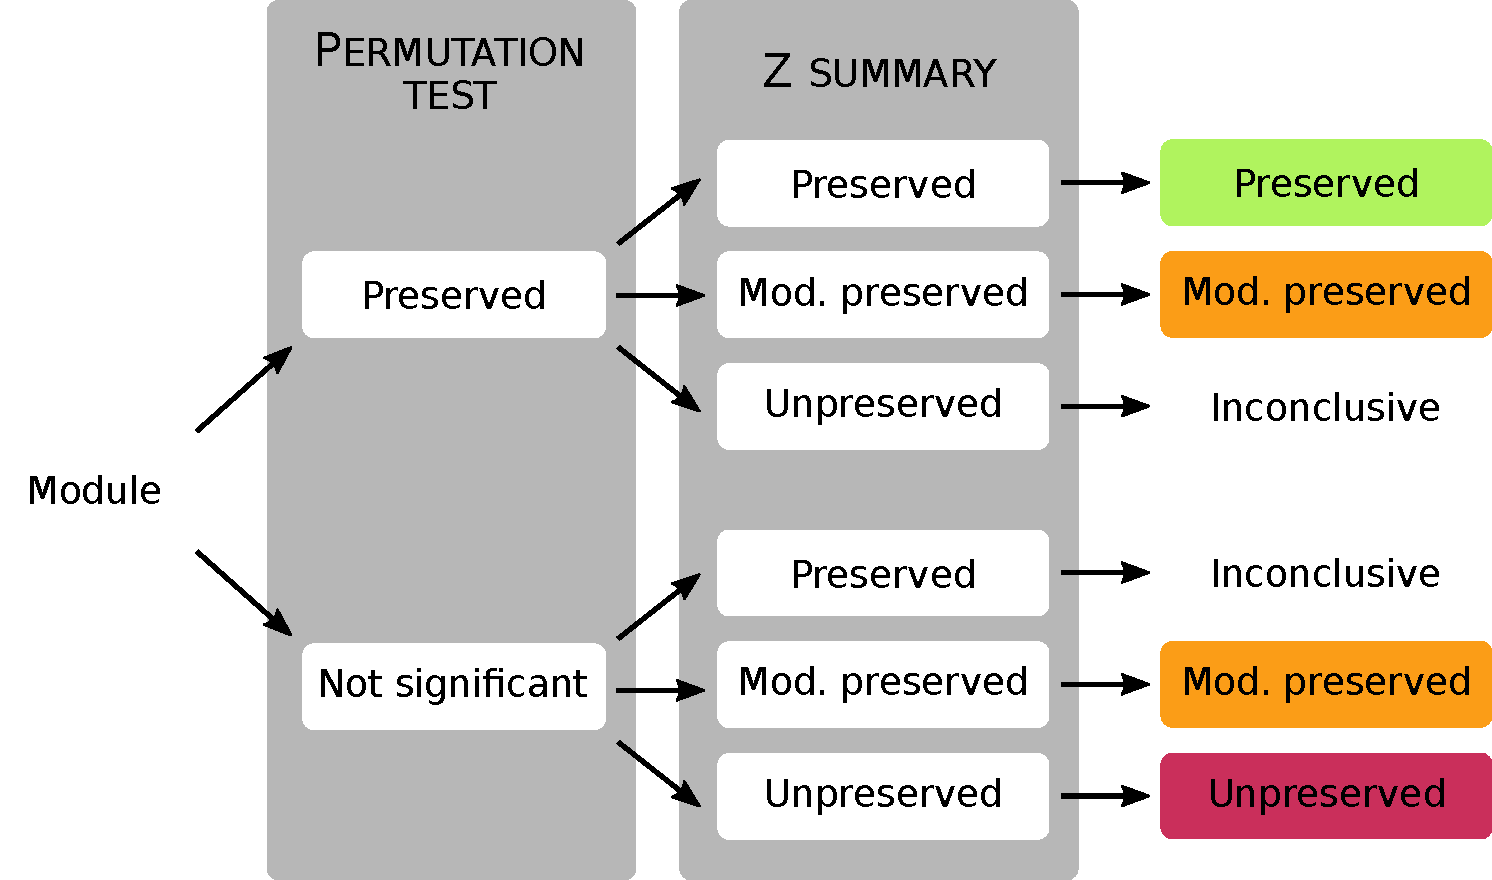
\includegraphics[width=\textwidth, center]{img/annexe_add_file_GWENA/additional_file_figure_1.pdf}
    \caption{Combination of the permutation test result ans the $Z_{summary}$ result in GWENA to return a final result on the module comparison.}
    \label{fig:supp_fig_comparison_schema_conclusion}
\end{figure}

%% ++++++++++++++++++++++++++++++++++++++++++++++++++++++++++++++++++++++++++++++++++++
%% +                                    Details data                                  +
%% ++++++++++++++++++++++++++++++++++++++++++++++++++++++++++++++++++++++++++++++++++++



\subsection{Details on case study data}
\label{supp:supp_detail_data_software}

Public data were obtained from GTEx v8 version on the GTEx Portal on 09/20/2020. 
Access to private data was subject to a request to dbGaP on accession number phs000424.v8.p2. Data were obtained on 10/21/2020.

\begin{table}[h!]
\begin{tabular}{ll}
\textbf{Data}      & \textbf{File}                                                     \\ \hline
Gene expression    & GTEx\_Analysis\_2017-06-05\_v8\_RNASeQCv1.1.9\_gene\_reads.gct.gz \\
Public annotation  & GTEx\_Analysis\_v8\_Annotations\_SampleAttributesDS.txt           \\
Private annotation & phs000424.v8.pht002742.v8.p2.c1.GTEx\_Subject\_Phenotypes.GRU.txt \\
Phenotype          & GTEx\_Analysis\_v8\_Annotations\_SubjectPhenotypesDS.txt         
\end{tabular}
\caption{Correspondence between file names and their contents}
% \label{}
\end{table}



%% ++++++++++++++++++++++++++++++++++++++++++++++++++++++++++++++++++++++++++++++++++++
%% +                                  PC-correction                                   +
%% ++++++++++++++++++++++++++++++++++++++++++++++++++++++++++++++++++++++++++++++++++++


\subsection{GTEx data normalization with PC-correction method}
\label{supp:supp_pc_correction}

In order to limit batch effect and handle the maximum of other co-founding effects, we chose to use a method based on PC-correction as recommended by Parsana et al. \cite{Parsana2019} for GTEx data. However age is usually included in this confounding factors, therefore is corrected. Since we're interested in gene changes we adapted the method to remove only the top $n$ PC correlated to age and which removed the least of genes correlating with age. The $n$ number of PC to remove was estimated by calculating the loss of correlation between phenotype and genes expression (Figure \ref{fig:supp_fig_ageing_correlation_density}) and confirmed by looking for the number of significantly correlated genes with two ageing gene databases (Figure \ref{fig:supp_fig_ageing_genes_overlapping}): GenAge \cite{Tacutu2018} and Digital Aging Atlas \cite{Craig2015}.

\begin{figure}[h!]
    % \centering
    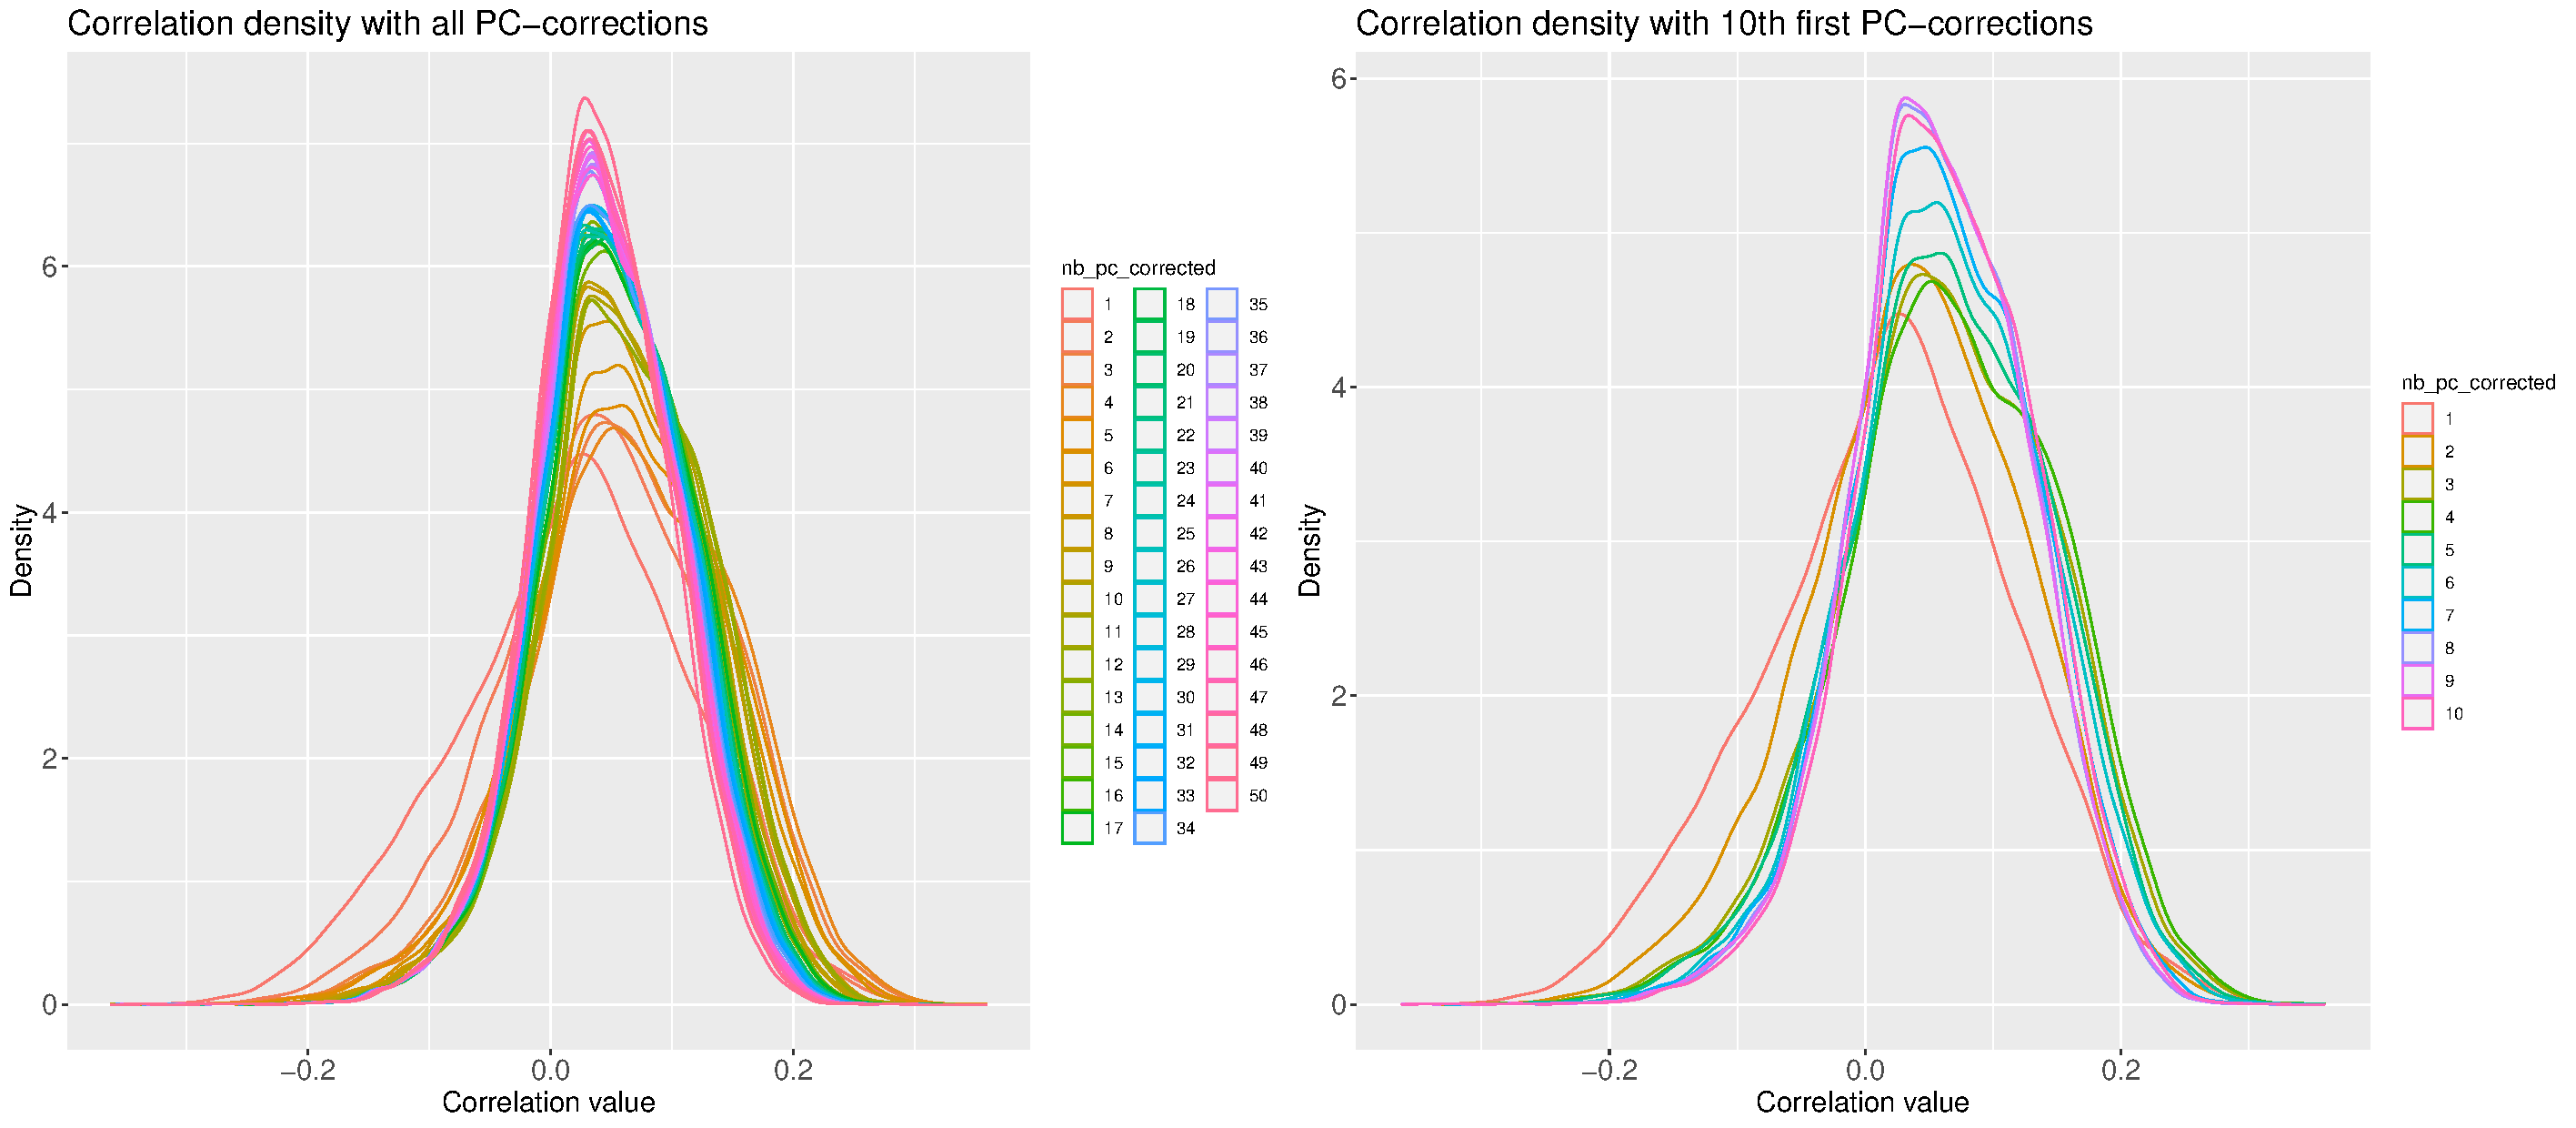
\includegraphics[width=\textwidth, center]{img/annexe_add_file_GWENA/additional_file_figure_2.pdf}
    \caption{Ageing genes correlation density with phenotype depending on the number of PC corrected. Left figure contains all PC correction tested. For clarity we filtered on the first 10 PC corrected on the right figure.}
    \label{fig:supp_fig_ageing_correlation_density}
\end{figure}

\begin{figure}[h!]
    % \centering
    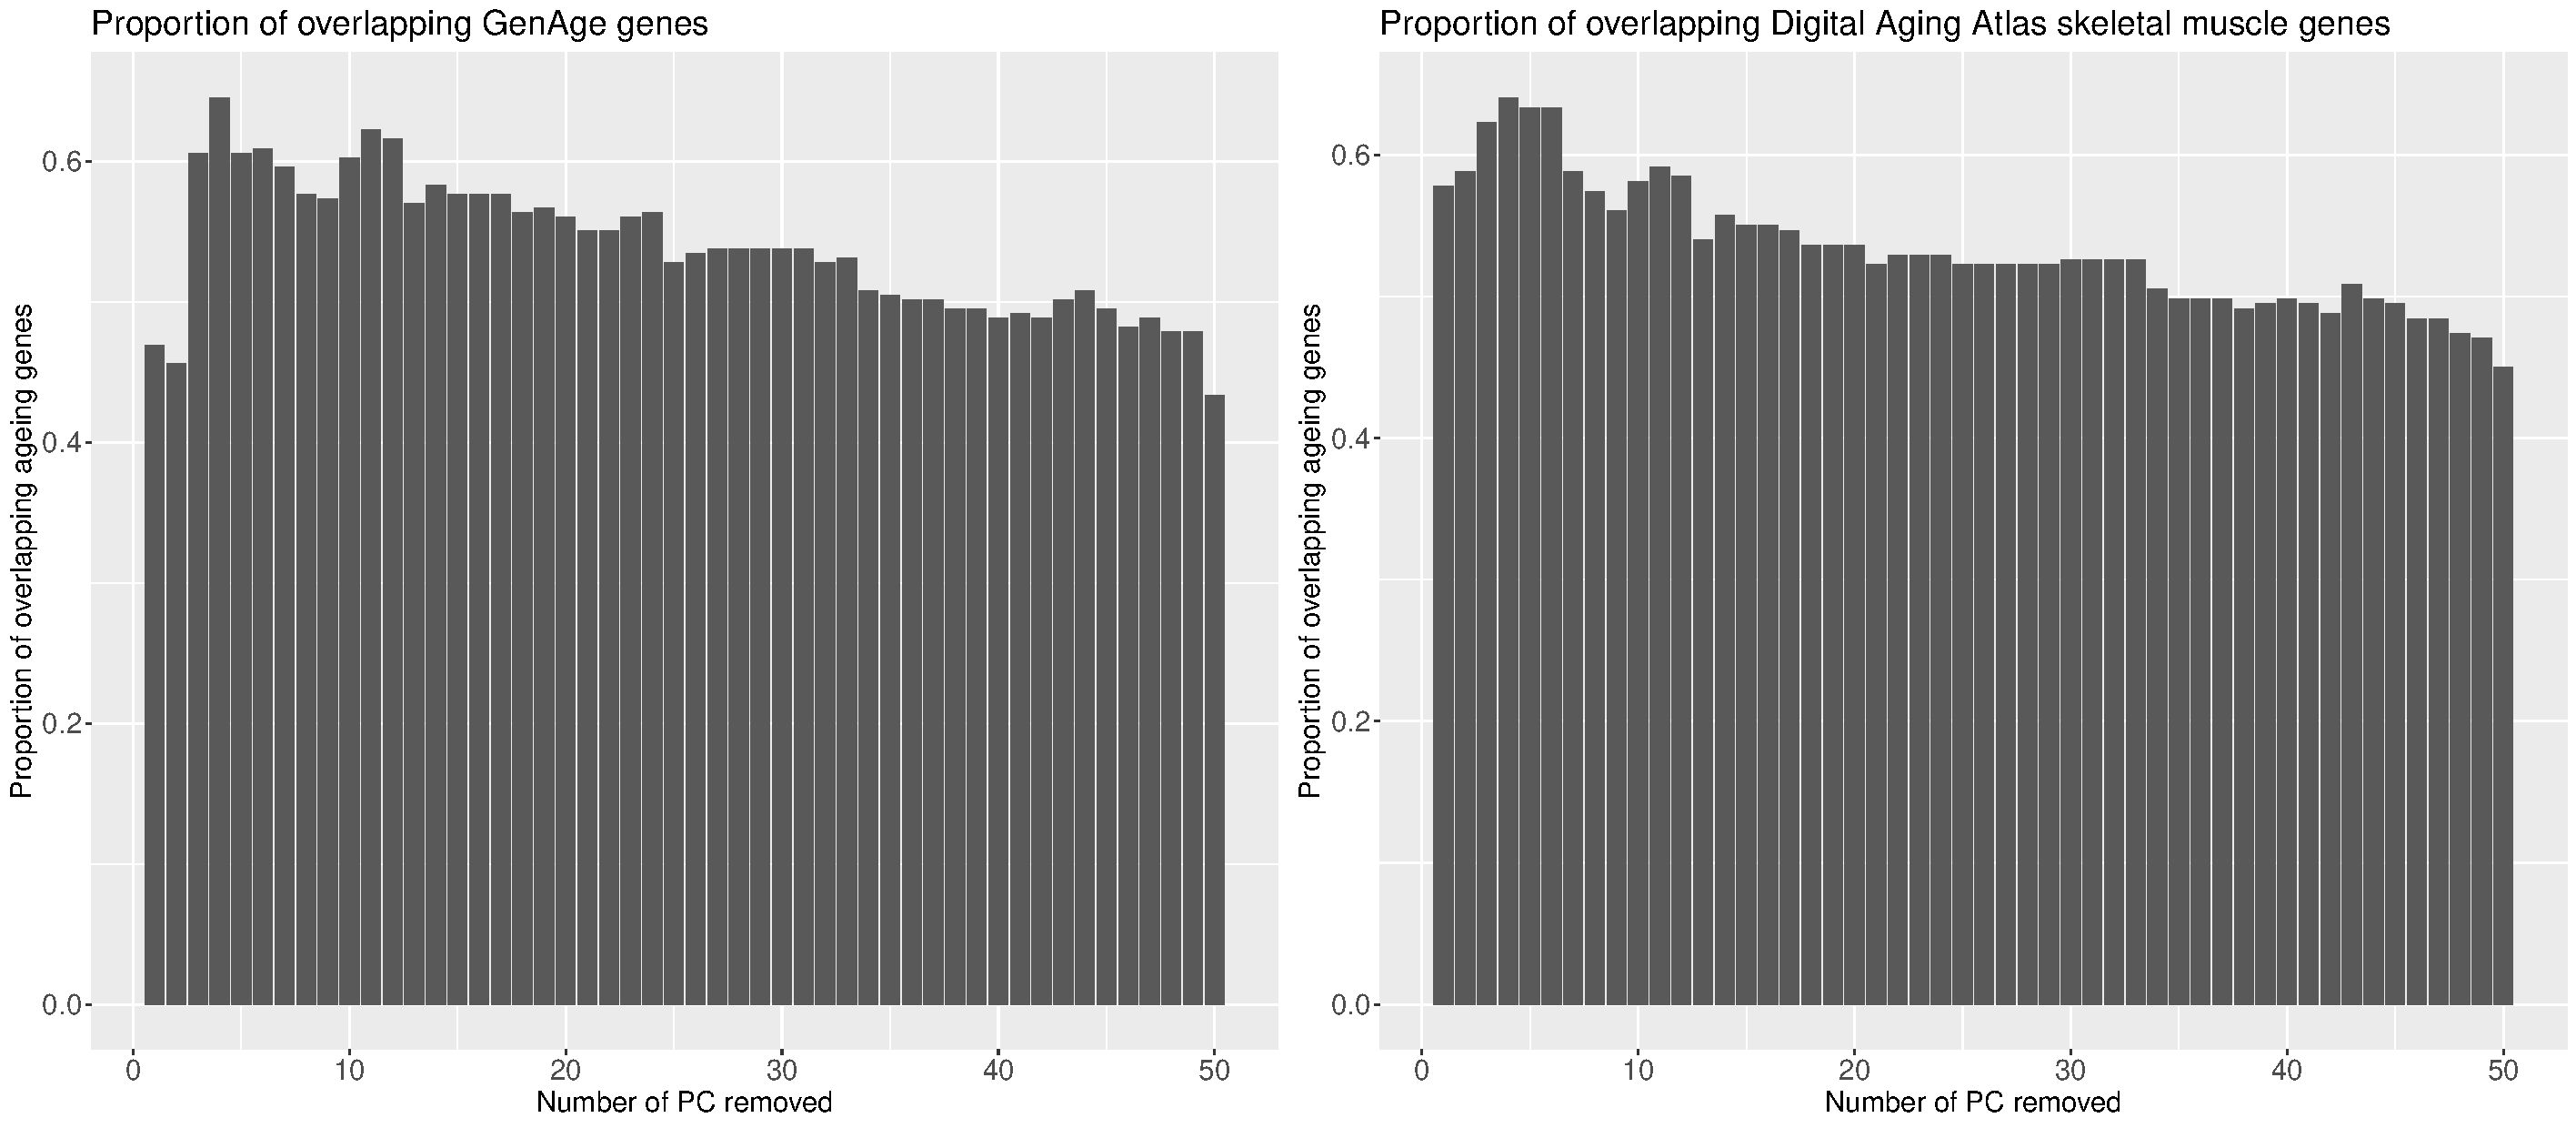
\includegraphics[width=\textwidth, center]{img/annexe_add_file_GWENA/additional_file_figure_3.pdf}
    \caption{Number of genes known to be associated with ageing.}
    \label{fig:supp_fig_ageing_genes_overlapping}
\end{figure}

Correlation density in Figure \ref{fig:supp_fig_ageing_correlation_density} suggest a similarity between the corrections from 2 to 5 PC removal. Combined with the proportion of overlapping known ageing genes in Figure \ref{fig:supp_fig_ageing_genes_overlapping} we determined the optimal number of PC $n$ to remove to be 4.

\clearpage
\section{Supplementary Results}
\subsection{Connectivity drop on all modules}
\label{supp:supp_connectivity_drop}

\begin{figure}[h!]
    \begin{adjustbox}{addcode=
        {\begin{minipage}{\width}}
        {
                \caption{Distribution of the connectivity for each gene by module between the two age range. Genes connectivity is ordered by increasing connectivity in the young condition (red).}
            \end{minipage}
        },rotate=90,center}
        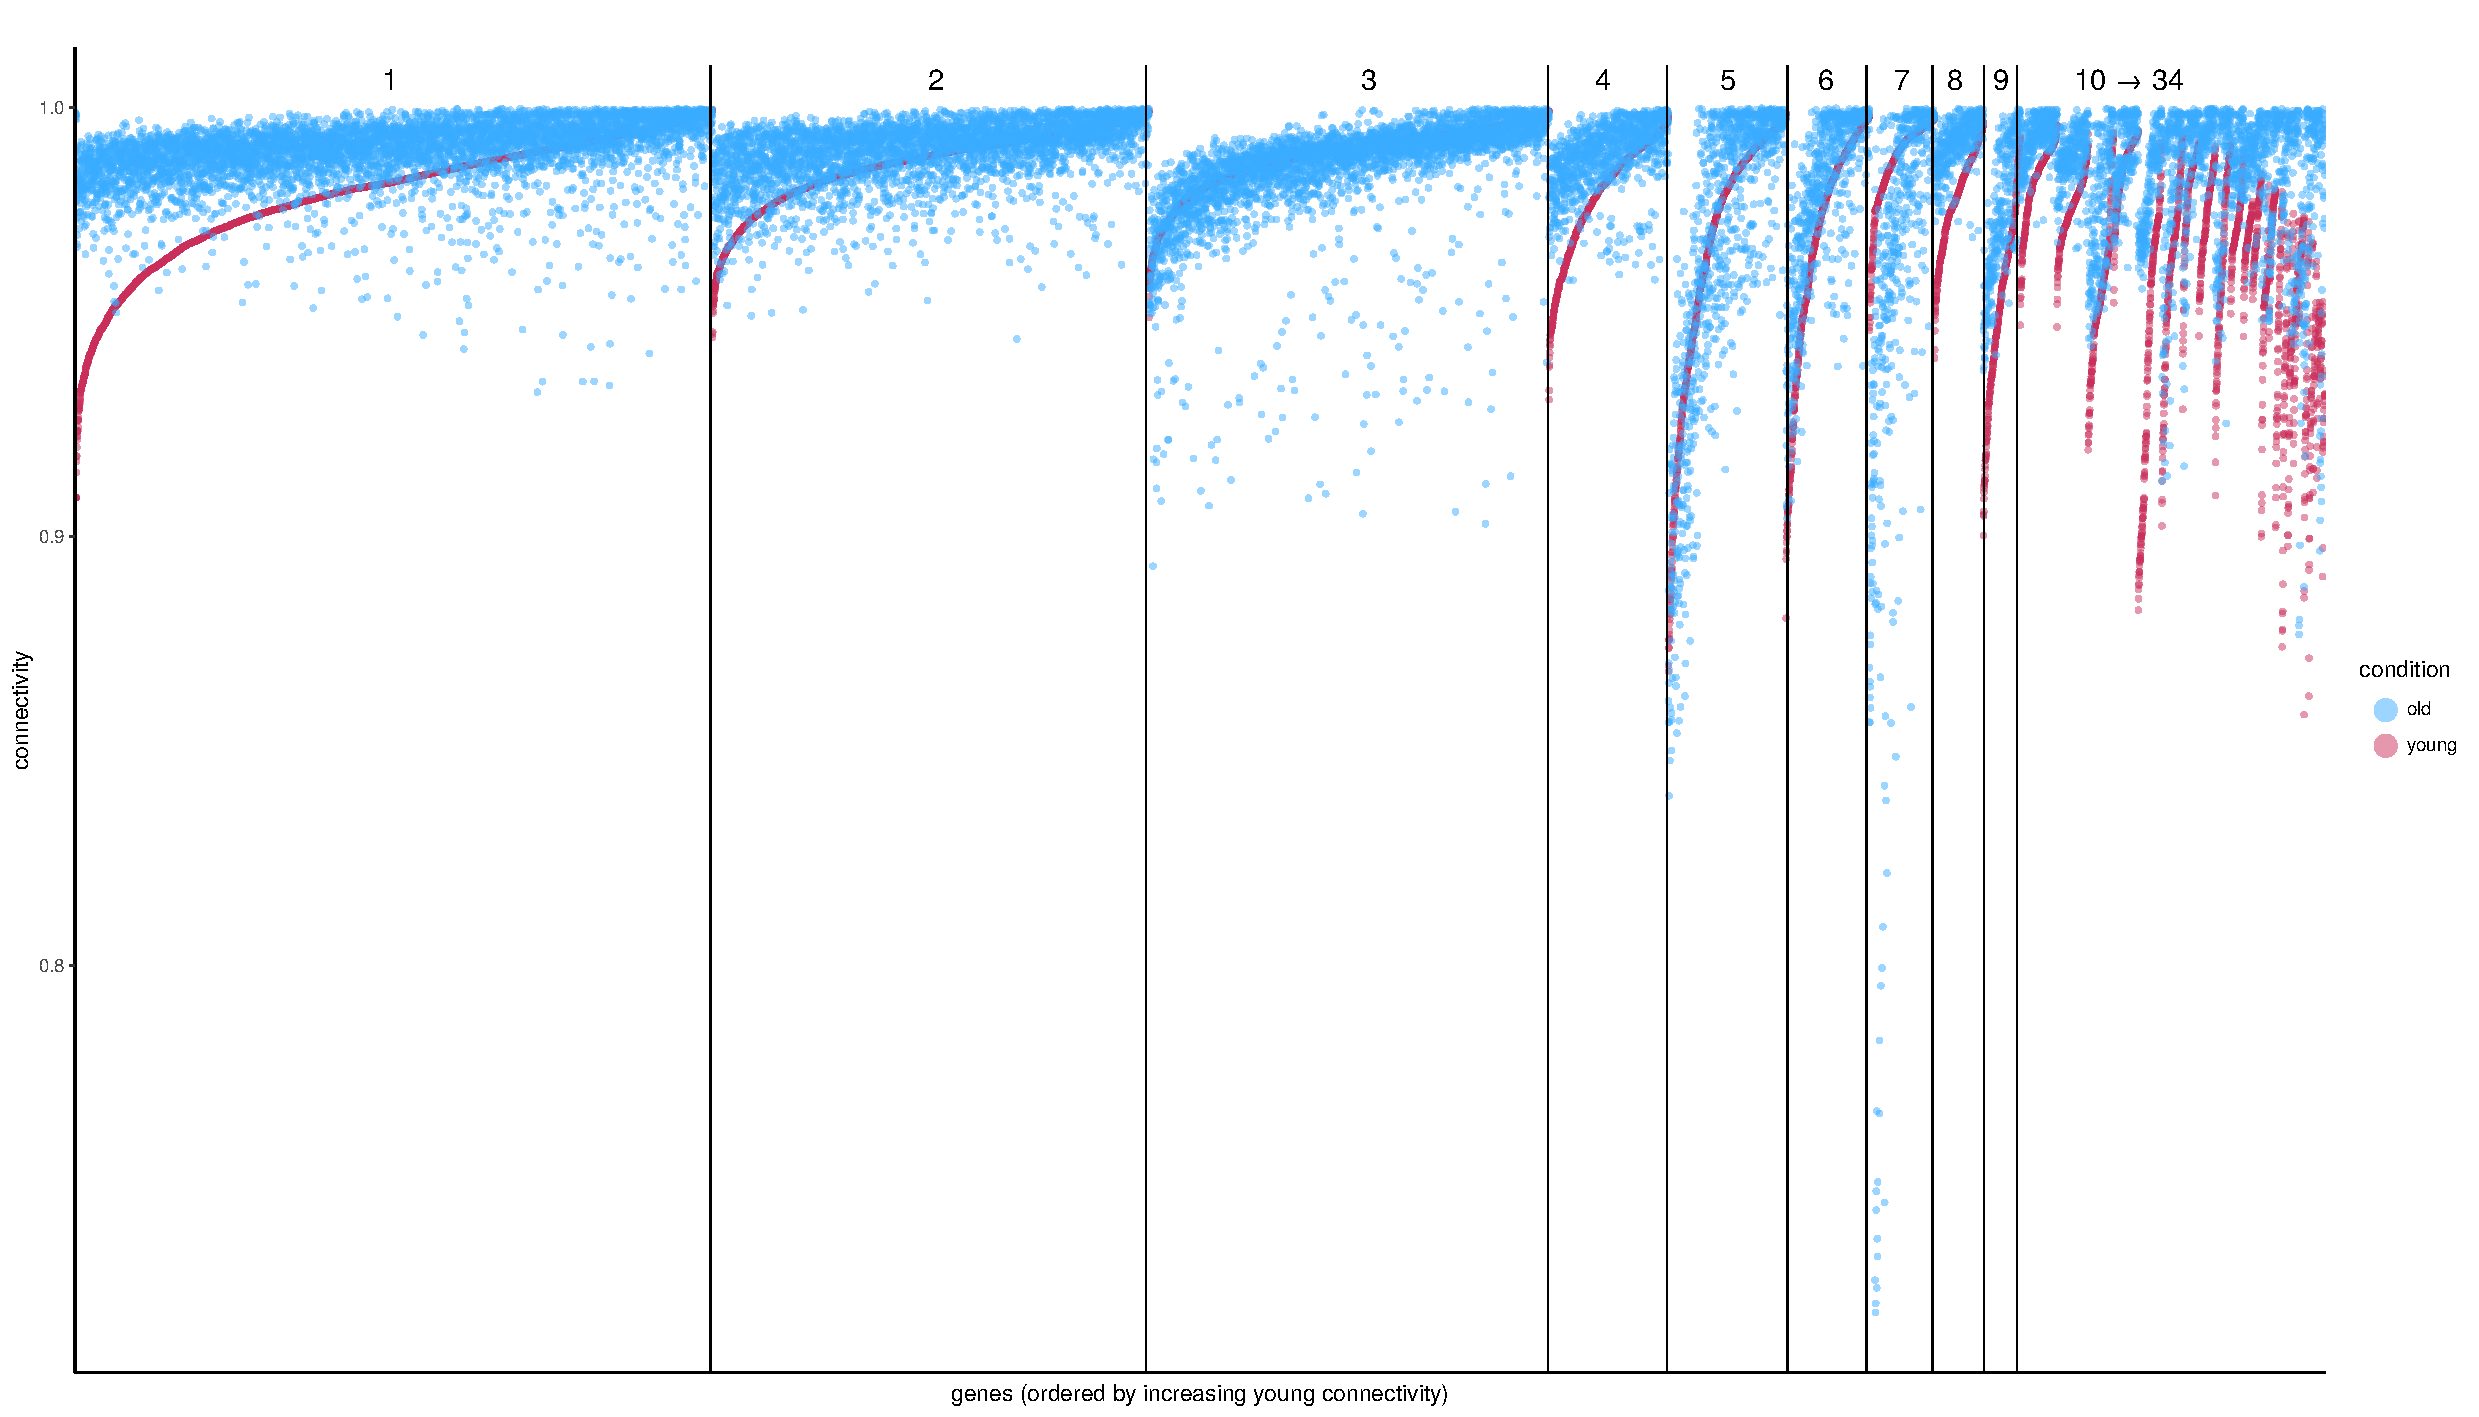
\includegraphics[scale=.476]{img/annexe_add_file_GWENA/additional_file_figure_4.pdf}%
    \end{adjustbox}
\end{figure}

\clearpage
\subsection{New enrichment terms in sub module 6 from module 7 old age range}
\label{supp:supp_sub_cluster_6_enrich_table}

% \resizebox{\textwidth}{!}{ % gneu gneu gneu marche pas
\LTcapwidth=\textwidth
% \setlength\LTright{3pt}
% \setlength\LTleft{0pt}
\begin{longtable}{@{}lp{5cm}lllp{5cm}l@{}}
\caption{Enrichment table from module 7 sub module 6 in old condition. Terms are sorted along their novelty (is the enrichment new compared to the enrichments from sub modules in the young age range) and then the source. Source is the enrichment database used on the gene set (GO:BP = Gene Ontology : Biological Process, GO:CC = Gene Ontology Cellular Compartment, GO:MF = Gene Ontology : Molecular Function, HP : Human Phenotype Ontology, WP = WikiPathway, KEGG = Kyoto Encyclopedia of Genes and Genomes, REAC = Reactome, TF = Transfac).}
\\ \hline
\textbf{source} & \textbf{term name}                                                                                                                & \textbf{is new} & \textbf{} & \textbf{source} & \textbf{term name}                                                                                                                                                    & \textbf{is new} \\ \hline
CORUM           & Fibrinogen complex                                                                                                                 & no               &           & GO:BP           & regulation of vasoconstriction                                                                                                                                         & yes              \\
GO:BP           & fibrinolysis                                                                                                                       & no               &           & GO:BP           & heterotypic cell-cell adhesion                                                                                                                                         & yes              \\
GO:BP           & negative regulation of blood coagulation                                                                                           & no               &           & GO:BP           & platelet aggregation                                                                                                                                                   & yes              \\
GO:BP           & negative regulation of hemostasis                                                                                                  & no               &           & GO:BP           & regulation of endothelial cell apoptotic process                                                                                                                       & yes              \\
GO:BP           & negative regulation of coagulation                                                                                                 & no               &           & GO:BP           & endothelial cell apoptotic process                                                                                                                                     & yes              \\
GO:BP           & negative regulation of wound healing                                                                                               & no               &           & GO:BP           & protein processing                                                                                                                                                     & yes              \\
GO:BP           & negative regulation of response to wounding                                                                                        & no               &           & GO:BP           & cell-matrix adhesion                                                                                                                                                   & yes              \\
GO:BP           & regulation of body fluid levels                                                                                                    & no               &           & GO:BP           & positive regulation of response to wounding                                                                                                                            & yes              \\
GO:CC           & blood microparticle                                                                                                                & no               &           & GO:BP           & positive regulation of blood circulation                                                                                                                               & yes              \\
GO:CC           & platelet alpha granule lumen                                                                                                       & no               &           & GO:BP           & vasoconstriction                                                                                                                                                       & yes              \\
GO:CC           & platelet alpha granule                                                                                                             & no               &           & GO:BP           & regulation of vesicle-mediated transport                                                                                                                               & yes              \\
GO:CC           & collagen-containing extracellular matrix                                                                                           & no               &           & GO:BP           & cell adhesion                                                                                                                                                          & yes              \\
GO:CC           & fibrinogen complex                                                                                                                 & no               &           & GO:BP           & biological adhesion                                                                                                                                                    & yes              \\
GO:CC           & extracellular space                                                                                                                & no               &           & GO:BP           & homotypic cell-cell adhesion                                                                                                                                           & yes              \\
GO:CC           & extracellular exosome                                                                                                              & no               &           & GO:BP           & vascular process in circulatory system                                                                                                                                 & yes              \\
GO:CC           & extracellular vesicle                                                                                                              & no               &           & GO:BP           & extrinsic apoptotic signaling pathway via death domain receptors                                                                                                       & yes              \\
GO:CC           & extracellular organelle                                                                                                            & no               &           & GO:CC           & secretory granule lumen                                                                                                                                                & yes              \\
GO:CC           & extracellular region                                                                                                               & no               &           & GO:CC           & cytoplasmic vesicle lumen                                                                                                                                              & yes              \\
GO:CC           & secretory granule                                                                                                                  & no               &           & GO:CC           & vesicle lumen                                                                                                                                                          & yes              \\
GO:CC           & secretory vesicle                                                                                                                  & no               &           & GO:CC           & extracellular matrix                                                                                                                                                   & yes              \\
GO:CC           & vesicle                                                                                                                            & no               &           & GO:CC           & cell surface                                                                                                                                                           & yes              \\
GO:MF           & enzyme inhibitor activity                                                                                                          & no               &           & GO:CC           & endoplasmic reticulum lumen                                                                                                                                            & yes              \\
HP              & Splenic rupture                                                                                                                    & no               &           & GO:CC           & cytoplasmic vesicle                                                                                                                                                    & yes              \\
WP              & COVID-19, thrombosis and anticoagulation                                                                                           & no               &           & GO:CC           & intracellular vesicle                                                                                                                                                  & yes              \\
GO:BP           & platelet degranulation                                                                                                             & yes              &           & GO:CC           & chylomicron                                                                                                                                                            & yes              \\
GO:BP           & regulation of blood coagulation                                                                                                    & yes              &           & GO:CC           & very-low-density lipoprotein particle                                                                                                                                  & yes              \\
GO:BP           & regulation of hemostasis                                                                                                           & yes              &           & GO:CC           & triglyceride-rich plasma lipoprotein particle                                                                                                                          & yes              \\
GO:BP           & regulation of coagulation                                                                                                          & yes              &           & GO:CC           & external side of plasma membrane                                                                                                                                       & yes              \\
GO:BP           & regulation of wound healing                                                                                                        & yes              &           & GO:CC           & high-density lipoprotein particle                                                                                                                                      & yes              \\
GO:BP           & plasminogen activation                                                                                                             & yes              &           & GO:CC           & plasma lipoprotein particle                                                                                                                                            & yes              \\
GO:BP           & regulation of response to wounding                                                                                                 & yes              &           & GO:CC           & lipoprotein particle                                                                                                                                                   & yes              \\
GO:BP           & protein activation cascade                                                                                                         & yes              &           & GO:CC           & protein-lipid complex                                                                                                                                                  & yes              \\
GO:BP           & blood coagulation, fibrin clot formation                                                                                           & yes              &           & GO:MF           & signaling receptor binding                                                                                                                                             & yes              \\
GO:BP           & vesicle-mediated transport                                                                                                         & yes              &           & GO:MF           & chaperone binding                                                                                                                                                      & yes              \\
GO:BP           & regulated exocytosis                                                                                                               & yes              &           & GO:MF           & immunoglobulin binding                                                                                                                                                 & yes              \\
GO:BP           & negative regulation of fibrinolysis                                                                                                & yes              &           & GO:MF           & lipoprotein particle receptor binding                                                                                                                                  & yes              \\
GO:BP           & exocytosis                                                                                                                         & yes              &           & GO:MF           & extracellular matrix structural constituent                                                                                                                            & yes              \\
GO:BP           & zymogen activation                                                                                                                 & yes              &           & HP              & Menometrorrhagia                                                                                                                                                       & yes              \\
GO:BP           & blood coagulation                                                                                                                  & yes              &           & HP              & Abnormality of the common coagulation pathway                                                                                                                          & yes              \\
GO:BP           & hemostasis                                                                                                                         & yes              &           & HP              & Spontaneous abortion                                                                                                                                                   & yes              \\
GO:BP           & coagulation                                                                                                                        & yes              &           & HP              & Abnormality of coagulation                                                                                                                                             & yes              \\
GO:BP           & regulation of fibrinolysis                                                                                                         & yes              &           & HP              & Hypofibrinogenemia                                                                                                                                                     & yes              \\
GO:BP           & positive regulation of heterotypic cell-cell adhesion                                                                              & yes              &           & HP              & Abnormality of circulating fibrinogen                                                                                                                                  & yes              \\
GO:BP           & regulation of cell-substrate adhesion                                                                                              & yes              &           & HP              & Joint swelling                                                                                                                                                         & yes              \\
GO:BP           & negative regulation of response to external stimulus                                                                               & yes              &           & HP              & Abnormality of the coagulation cascade                                                                                                                                 & yes              \\
GO:BP           & negative regulation of blood vessel diameter                                                                                       & yes              &           & HP              & Abnormal delivery                                                                                                                                                      & yes              \\
GO:BP           & negative regulation of response to stimulus                                                                                        & yes              &           & HP              & Abnormal thrombosis                                                                                                                                                    & yes              \\
GO:BP           & regulation of heterotypic cell-cell adhesion                                                                                       & yes              &           & KEGG            & Complement and coagulation cascades                                                                                                                                    & yes              \\
GO:BP           & positive regulation of blood coagulation                                                                                           & yes              &           & KEGG            & Platelet activation                                                                                                                                                    & yes              \\
GO:BP           & positive regulation of hemostasis                                                                                                  & yes              &           & KEGG            & Cholesterol metabolism                                                                                                                                                 & yes              \\
GO:BP           & positive regulation of coagulation                                                                                                 & yes              &           & MIRNA           & hsa-miR-409-3p                                                                                                                                                         & yes              \\
GO:BP           & wound healing                                                                                                                      & yes              &           & MIRNA           & hsa-miR-144-3p                                                                                                                                                         & yes              \\
GO:BP           & negative regulation of multicellular organismal process                                                                            & yes              &           & REAC            & Platelet degranulation                                                                                                                                                 & yes              \\
GO:BP           & positive regulation of cell-substrate adhesion                                                                                     & yes              &           & REAC            & Response to elevated platelet cytosolic Ca2+                                                                                                                           & yes              \\
GO:BP           & secretion by cell                                                                                                                  & yes              &           & REAC            & Platelet activation, signaling and aggregation                                                                                                                         & yes              \\
GO:BP           & negative regulation of endothelial cell apoptotic process                                                                          & yes              &           & REAC            & Regulation of Insulin-like Growth Factor (IGF) transport and uptake by Insulin-like Growth Factor Binding Proteins (IGFBPs) & yes              \\
GO:BP           & positive regulation of vasoconstriction                                                                                            & yes              &           & REAC            & Post-translational protein phosphorylation                                                                                                                             & yes              \\
GO:BP           & export from cell                                                                                                                   & yes              &           & REAC            & Hemostasis                                                                                                                                                             & yes              \\
GO:BP           & negative regulation of cellular process                                                                                            & yes              &           & REAC            & GRB2:SOS provides linkage to MAPK signaling for Integrins                                                                                                              & yes              \\
GO:BP           & regulation of response to stress                                                                                                   & yes              &           & REAC            & p130Cas linkage to MAPK signaling for integrins                                                                                                                        & yes              \\
GO:BP           & positive regulation of substrate adhesion-dependent cell spreading                      & yes              &           & REAC            & Regulation of TLR by endogenous ligand                                                                                                                                 & yes              \\
GO:BP           & regulation of blood vessel diameter                                                                                                & yes              &           & REAC            & Common Pathway of Fibrin Clot Formation                                                                                                                                & yes              \\
GO:BP           & regulation of tube diameter                                                                                                        & yes              &           & REAC            & Integrin signaling                                                                                                                                                     & yes              \\
GO:BP           & negative regulation of extrinsic apoptotic signaling pathway via death domain receptors & yes              &           & REAC            & Signaling by high-kinase activity BRAF mutants                                                                                                                         & yes              \\
GO:BP           & regulation of tube size                                                                                                            & yes              &           & REAC            & Platelet Aggregation (Plug Formation)                                                                                                                                  & yes              \\
GO:BP           & cell-substrate adhesion                                                                                                            & yes              &           & REAC            & Formation of Fibrin Clot (Clotting Cascade)                                                                                                                            & yes              \\
GO:BP           & post-translational protein modification                                                                                            & yes              &           & REAC            & MAP2K and MAPK activation                                                                                                                                              & yes              \\
GO:BP           & response to wounding                                                                                                               & yes              &           & REAC            & Signaling by moderate kinase activity BRAF mutants                                                                                                                     & yes              \\
GO:BP           & secretion                                                                                                                          & yes              &           & REAC            & Signaling downstream of RAS mutants                                                                                                                                    & yes              \\
GO:BP           & regulation of response to external stimulus                                                                                        & yes              &           & REAC            & Paradoxical activation of RAF signaling by kinase inactive BRAF                                                                                                        & yes              \\
GO:BP           & platelet activation                                                                                                                & yes              &           & REAC            & Signaling by RAS mutants                                                                                                                                               & yes              \\
GO:BP           & transport                                                                                                                          & yes              &           & REAC            & Signaling by BRAF and RAF fusions                                                                                                                                      & yes              \\
GO:BP           & response to stress                                                                                                                 & yes              &           & REAC            & Oncogenic MAPK signaling                                                                                                                                               & yes              \\
GO:BP           & establishment of localization                                                                                                      & yes              &           & REAC            & Dissolution of Fibrin Clot                                                                                                                                             & yes              \\
GO:BP           & negative regulation of epithelial cell apoptotic process                                                                           & yes              &           & REAC            & Integrin cell surface interactions                                                                                                                                     & yes              \\
GO:BP           & regulation of cell adhesion                                                                                                        & yes              &           & TF              & Factor: HNF1A; motif: GGTTAATNATTAMC                                                                                                                                   & yes              \\
GO:BP           & regulation of substrate adhesion-dependent cell spreading                                                                          & yes              &           & TF              & Factor: HNF-1alpha; motif: GGTTAATNWTTAMCN                                                                                                                             & yes              \\
GO:BP           & induction of bacterial agglutination                                                                                               & yes              &           & TF              & Factor: Sox-2; motif: NNNNNAACAAWGN; match class: 1                                                                                                                    & yes              \\
GO:BP           & regulation of response to stimulus                                                                                                 & yes              &           & WP              & Folate Metabolism                                                                                                                                                      & yes              \\
GO:BP           & proteolysis                                                                                                                        & yes              &           & WP              & Selenium Micronutrient Network                                                                                                                                         & yes              \\
GO:BP           & negative regulation of biological process                                                                                          & yes              &           & WP              & Human Complement System                                                                                                                                                & yes              \\
GO:BP           & regulation of cell-cell adhesion                                                                                                   & yes              &           & WP              & Blood Clotting Cascade                                                                                                                                                 & yes              \\
GO:BP           & regulation of extrinsic apoptotic signaling pathway via death domain receptors          & yes              &           & WP              & Fibrin Complement Receptor 3 Signaling Pathway                                                                                                                         & yes              \\
GO:BP           & positive regulation of wound healing                                                                                               & yes              &           & WP              & Vitamin B12 Metabolism                                                                                                                                                 & yes             

\label{supp:table_c6_enrich}
\end{longtable}


The distribution of the newly and previously found terms in the enrichment analysis across the the sub-modules from young and old age range (Figure \ref{fig:supp_fig_upset_subclusters_enrichments}).

\begin{figure}[h!]
    % \centering
    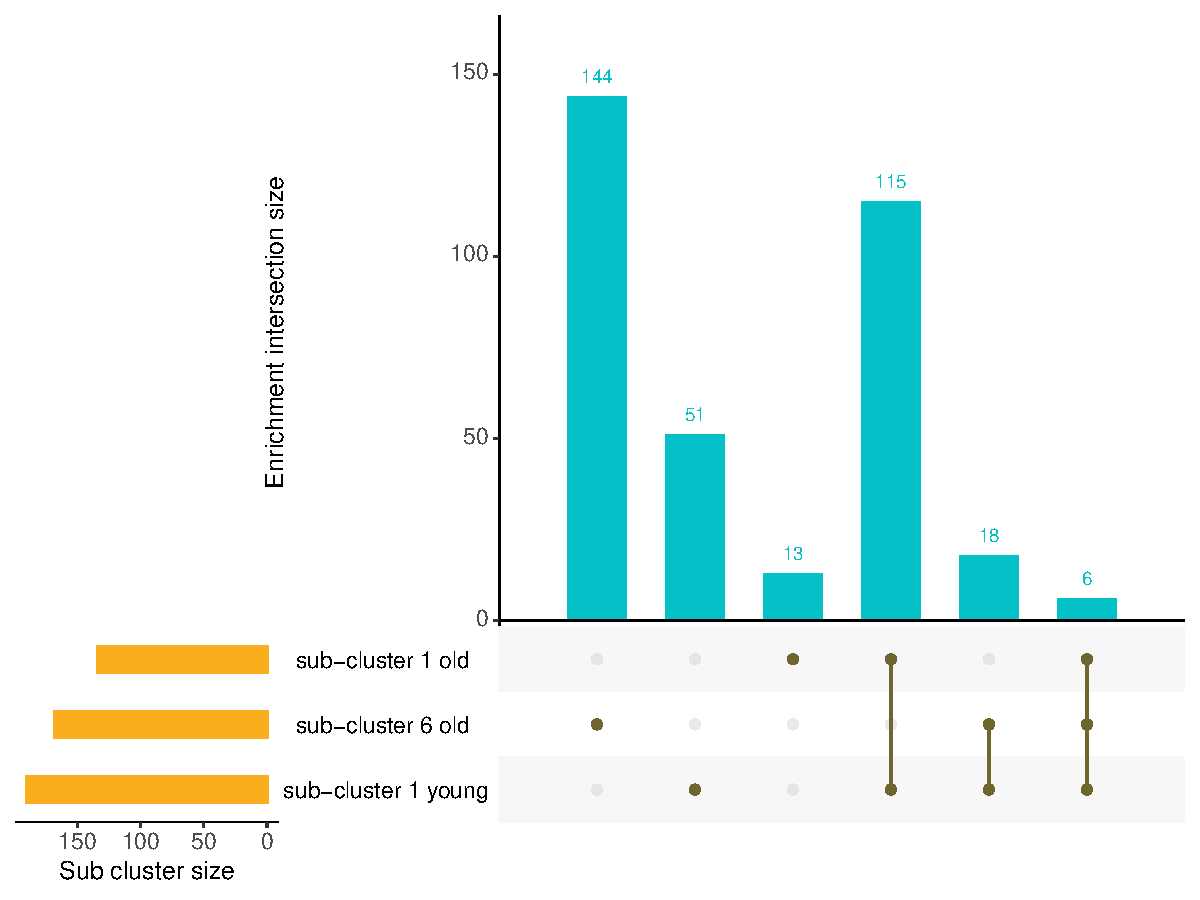
\includegraphics[width=\textwidth, center]{img/annexe_add_file_GWENA/additional_file_figure_5.pdf}
    \caption{Overlap between the enrichments found in sub-cluster 1 young, sub-cluster 1 old, and sub-cluster 6 old.(Upset diagram)}
    \label{fig:supp_fig_upset_subclusters_enrichments}
\end{figure} 


% \hfill \break
% \clearpage
% \bibliographystyle{unsrt}
% \bibliography{additional_file_1}
    \chapter{NetRep statistics detail}


\todo{TODO : récupérer, résumer (et traduire ?) l'explication et l'interprétation biologique des 7 métriques disponibles dans les Supplemental Experimental Procedures de la publication de netrep (https://doi.org/10.1016/j.cels.2016.06.012)}

Source : Document S1. Supplemental Experimental Procedures, Figures S1–S7, and Tables S1–S4, S6, and S7 from 

    \chapter{Demande d'accès dbGaP aux données protégées de GTEx}

\label{annexe:dbgap}

\section{Query title}
Muscle gene co-expression in multiple age range for sarcopenia condition exploration

\section{Research use statement}
As a multi factorial phenomena, aging is a complex condition to study. Current analysis of transcriptomic data joined with phenotypic ones have unravel few genes and environmental variables impacting it. However, aging remains not fully understood. These may come from current approaches focusing on single factors while aging is more about interaction between many of them. This is why we would like to study it through the spectrum of the co-expression networks. However, because aging is already complex by itself, we will focus on a single tissue in the beginning : muscle. Reasons are myopenia and dynapenia (known together as sarcopenia) are responsible for loss of autonomy, weak metabolic aggression resistance, and increased mortality.
By using our yet to be published pipeline developed in our lab, we aim to build gene co-expression modules and network from transcriptomic data and characterize them with external resources. This pipeline begin with a quality assessment of the data, based on the technique used to get transcriptomic information (either microarray or RNA-Seq). It then compute co-expression levels and detects modules by using the WGCNA package. Additionnal steps are then performed to fully charachterize the modules : biological enrichment, topological study, phenotipic association, differentially expressed and condition-specific gene positionning.The external resources used to it include : enrichment databases (GO, KEGG, etc.), phenotypic information (exact age, condition of death, ethnicity), and age related databases (Digital aging atlas, Aging map, etc.). The use of these complementary information represents no additional risk to participants since only summarized gene information we'll be used in the form of modules. No other raw transcriptomics data will be combined to the GTEx data, but only a comparison of the modules built on each datasets in order to study the reproductibility of our modules, and the comparison with modules built on sarcopenia dedicated datasets.
Phenotipyc information is the main reason for our current demand regarding protected datasets because we think precise age and cause of death will impact the aging expression. 
No collaboration with other institution is planned.
Finnally, this methodological work will advance the understanding of the genetic bases of the aging processes occurring in the muscle.


\section{Non-technical summary}
Aging affect every one of us. It is defined as the progressive degradation of biological functions inside the body. In the muscle, this results in a decreasing in muscle density and strength called sarcopenia. They are responsible for mobility difficulties, therefore autonomy, and a deficit in body protection against aggression, sometimes leading to death. With this risks at stake, it is understandable that a better understanding of aging processes in muscle is important for public health. Few single genes linked to it have already been discovered, however we still don't fully understand the mechanisms occurring and how to limit them. Gene expression is a witness of the changes in the body mechanisms. By studying the expression of the genes and the coordination between this levels of expression, therefore patterns of expression, we aim to detect news genes involved in muscle aging. Do to so, we regroup the most coordinated genes in entities called module and try to unravel the biological interactions which link them. Because some of this genes are already involved into other biological interactions, we can have an insight on the regulations that take place in this case by extrapolating information. These, will lead to the discovery of new genes associated with sarcopenia.

\hfill \break
\textit{Réalisé le 30/09/2019}

\textcolor[RGB]{220,220,220}{\rule{\linewidth}{0.2pt}}

\section{Access update : Research Progress}
Current analysis of the GTEx data focused on the skeletal muscle samples as we are studying sarcopenia and other aging impact on muscle. The RNAseq data was then split in two opposite age range (young and old) to emphase and capture the differences in aging through our newly developped differential gene co-expression network pipeline GWENA (\url{https://www.bioconductor.org/packages/release/bioc/html/GWENA.html}). 
A first analysis solely on the modules (gene groups) detected by GWENA in the young condition. A selection of interesting modules for muscle activity was achieved through a combinaison of moduels phenotypic association and gene sets enrichment. Inside one promissing module, hub genes connected in the network to genes involved in muscle activity allowed the identification of genes with strong evidence of contribution to muscle developpemnt and growth.
A second analysis used the full potential of the differential co-expression analysis offered by GWENA to find specific co-expression modules to aging. Important topological variation lead us to focus on one module. Further investigation is currently underway to characterise the origin of the specificity and this variations. 

\hfill \break
\textit{Réalisé le 01/12/2020}

    \chapter{Enrichissements des intersections de gènes en chapitre 2}
\label{annexe:chap_2_genes_intersect_enrichments}

Résultats des tests d'enrichissement effectués grâce à GWENA sur les intersections ayant au moins 3 tissus et 5 gènes lors du chapitre \ref{chapter:multidim}. Pour rappel :
\begin{itemize}
    \item{\textbf{GO} : Gene Ontology}
    \item{\textbf{GO:MF} : GO Molecular Function}
    \item{\textbf{GO:BP} : GO Biological Process}
    \item{\textbf{GO:CC} : GO Cellular Compartment}
    \item{\textbf{KEGG} : Kyoto Encyclopedia of Genes and Genomes}
    \item{\textbf{REAC} : Reactome}
    \item{\textbf{WP} : WikiPathway}
    \item{\textbf{TF} : TRANSFAC}
    \item{\textbf{MIRNA} : mirTarBase}
    \item{\textbf{HPA} : Human Protein Atlas}
    \item{\textbf{CORUM} : Comprehensive Resource of Mammalian protein complexes}
    \item{\textbf{HP} : Human Phenotype Ontology}
\end{itemize}


\section*{esophagus\_muscularis\_mod\_pres \newline skin\_sun\_exposed\_mod\_pres \newline thyroid\_mod\_pres}

\begin{longtable}{ll}
\toprule
Source & Nom du terme enrichit\\
\midrule
CORUM & Cell-cell junction complex (ARHGAP10-CTNNA1)\\
GO:BP & dicarboxylic acid catabolic process\\
HP & Hypoglutaminemia\\
HP & Abnormal CSF glutamine family amino acid concentration\\
HP & Abnormal CSF glutamine concentration\\
HP & Decreased CSF glutamine concentration\\
\bottomrule
\end{longtable}

\section*{esophagus\_muscularis\_mod\_pres \newline nerve\_tibial\_mod\_pres \newline skin\_sun\_exposed\_mod\_pres}

\begin{longtable}{ll}
\toprule
Source & Nom du terme enrichit\\
\midrule
CORUM & Seipin-lipin1 complex\\
GO:BP & adenosine to inosine editing\\
GO:BP & base conversion or substitution editing\\
GO:MF & phenylethanolamine N-methyltransferase activity\\
GO:MF & creatine:sodium symporter activity\\
GO:MF & XTP binding\\
GO:MF & ITP binding\\
\bottomrule
\end{longtable}

\section*{esophagus\_muscularis\_mod\_pres \newline nerve\_tibial\_mod\_pres \newline skin\_sun\_exposed\_mod\_pres \newline thyroid\_mod\_pres}

\begin{longtable}{ll}
\toprule
Source & Nom du terme enrichit\\
\midrule
GO:MF & dGTPase activity\\
GO:MF & triphosphoric monoester hydrolase activity\\
GO:MF & guanyl deoxyribonucleotide binding\\
GO:MF & dGTP binding\\
HPA & skin 1; melanocytes[High]\\
HPA & testis; peritubular cells[High]\\
\bottomrule
\end{longtable}

\section*{esophagus\_mucosa\_mod\_pres \newline skin\_not\_sun\_exposed\_mod\_pres \newline skin\_sun\_exposed\_mod\_pres}

\begin{longtable}{ll}
\toprule
Source & Nom du terme enrichit\\
\midrule
GO:BP & melanin biosynthetic process\\
GO:BP & melanin metabolic process\\
GO:BP & secondary metabolite biosynthetic process\\
GO:BP & phenol-containing compound biosynthetic process\\
GO:BP & secondary metabolic process\\
GO:BP & pigment biosynthetic process\\
GO:BP & pigment metabolic process\\
GO:BP & pigmentation\\
GO:BP & phenol-containing compound metabolic process\\
GO:BP & regulation of secondary metabolic process\\
GO:BP & regulation of melanin biosynthetic process\\
GO:BP & regulation of secondary metabolite biosynthetic process\\
GO:MF & melanin-concentrating hormone receptor activity\\
HPA & retina; pigment epithelial cells[High]\\
\bottomrule
\end{longtable}

\section*{esophagus\_mucosa\_mod\_pres \newline muscle\_skeletal\_mod\_pres \newline thyroid\_mod\_pres}

\begin{longtable}{ll}
\toprule
Source & Nom du terme enrichit\\
\midrule
GO:BP & oxygen transport\\
GO:BP & gas transport\\
GO:BP & hydrogen peroxide catabolic process\\
GO:CC & hemoglobin complex\\
GO:CC & haptoglobin-hemoglobin complex\\
GO:MF & hemoglobin binding\\
GO:MF & haptoglobin binding\\
GO:MF & oxygen carrier activity\\
GO:MF & oxygen binding\\
GO:MF & peroxidase activity\\
GO:MF & oxidoreductase activity, acting on peroxide as acceptor\\
GO:MF & molecular carrier activity\\
\bottomrule
\end{longtable}

\section*{esophagus\_mucosa\_mod\_pres \newline muscle\_skeletal\_mod\_pres \newline skin\_sun\_exposed\_mod\_pres}

\begin{longtable}{ll}
\toprule
Source & Nom du terme enrichit\\
\midrule
GO:BP & response to nicotine\\
GO:MF & V1B vasopressin receptor binding\\
REAC & ADORA2B mediated anti-inflammatory cytokines production\\
\bottomrule
\end{longtable}

\section*{esophagus\_mucosa\_mod\_pres \newline muscle\_skeletal\_unpres \newline skin\_sun\_exposed\_mod\_pres}

\begin{longtable}{ll}
\toprule
Source & Nom du terme enrichit\\
\midrule
HP & Gonadal tissue inappropriate for external genitalia or chromosomal sex\\
\bottomrule
\end{longtable}

\section*{artery\_tibial\_mod\_pres \newline skin\_not\_sun\_exposed\_mod\_pres \newline skin\_sun\_exposed\_mod\_pres}

\begin{longtable}{ll}
\toprule
Source & Nom du terme enrichit\\
\midrule
GO:MF & neuropeptide receptor activity\\
\bottomrule
\end{longtable}

\section*{artery\_tibial\_mod\_pres \newline esophagus\_muscularis\_mod\_pres \newline thyroid\_mod\_pres}

\begin{longtable}{ll}
\toprule
Source & Nom du terme enrichit\\
\midrule
GO:BP & response to corticotropin-releasing hormone\\
GO:BP & cellular response to corticotropin-releasing hormone stimulus\\
GO:BP & regulation of type B pancreatic cell proliferation\\
GO:BP & type B pancreatic cell proliferation\\
GO:CC & transcription regulator complex\\
GO:CC & chromatin\\
GO:MF & DNA-binding transcription activator activity, RNA polymerase II-specific\\
GO:MF & DNA-binding transcription activator activity\\
GO:MF & glucocorticoid receptor binding\\
GO:MF & nuclear receptor activity\\
GO:MF & ligand-activated transcription factor activity\\
GO:MF & DNA-binding transcription factor activity, RNA polymerase II-specific\\
GO:MF & DNA-binding transcription factor activity\\
GO:MF & steroid hormone receptor binding\\
TF & Factor: ATF; motif: CNSTGACGTNNNYC; match class: 1\\
\bottomrule
\end{longtable}

\section*{artery\_tibial\_mod\_pres \newline esophagus\_mucosa\_mod\_pres \newline thyroid\_mod\_pres}
No enrichment found

\section*{artery\_tibial\_mod\_pres \newline esophagus\_mucosa\_mod\_pres \newline skin\_sun\_exposed\_mod\_pres}

\begin{longtable}{ll}
\toprule
Source & Nom du terme enrichit\\
\midrule
GO:BP & positive regulation of gastrulation\\
GO:BP & primitive streak formation\\
GO:BP & regulation of gastrulation\\
KEGG & Viral protein interaction with cytokine and cytokine receptor\\
\bottomrule
\end{longtable}

\section*{artery\_tibial\_mod\_pres \newline esophagus\_mucosa\_mod\_pres \newline skin\_sun\_exposed\_unpres}
No enrichment found

\section*{artery\_tibial\_mod\_pres \newline esophagus\_mucosa\_mod\_pres \newline nerve\_tibial\_mod\_pres}

\begin{longtable}{ll}
\toprule
Source & Nom du terme enrichit\\
\midrule
GO:CC & blood microparticle\\
GO:CC & platelet alpha granule lumen\\
GO:CC & platelet alpha granule\\
GO:CC & collagen-containing extracellular matrix\\
GO:CC & extracellular matrix\\
GO:CC & external encapsulating structure\\
KEGG & Complement and coagulation cascades\\
REAC & Platelet degranulation\\
REAC & Response to elevated platelet cytosolic Ca2+\\
TF & Factor: C/EBP; motif: NTTRCNNAANNN\\
WP & Complement and Coagulation Cascades\\
\bottomrule
\end{longtable}

\section*{artery\_tibial\_mod\_pres \newline esophagus\_mucosa\_mod\_pres \newline nerve\_tibial\_mod\_pres \newline thyroid\_mod\_pres}

\begin{longtable}{ll}
\toprule
Source & Nom du terme enrichit\\
\midrule
CORUM & Fibrinogen complex\\
GO:BP & negative regulation of wound healing\\
GO:BP & plasminogen activation\\
GO:BP & negative regulation of response to wounding\\
GO:BP & fibrinolysis\\
GO:BP & blood coagulation, fibrin clot formation\\
GO:BP & protein activation cascade\\
GO:BP & platelet degranulation\\
GO:BP & regulation of wound healing\\
GO:BP & negative regulation of blood coagulation\\
GO:BP & regulation of response to wounding\\
GO:BP & negative regulation of hemostasis\\
GO:BP & negative regulation of coagulation\\
GO:BP & zymogen activation\\
GO:BP & regulation of blood coagulation\\
GO:BP & regulation of hemostasis\\
GO:BP & regulation of coagulation\\
GO:BP & positive regulation of heterotypic cell-cell adhesion\\
GO:BP & regulation of heterotypic cell-cell adhesion\\
GO:BP & negative regulation of response to external stimulus\\
GO:BP & positive regulation of vasoconstriction\\
GO:BP & negative regulation of endothelial cell apoptotic process\\
GO:BP & negative regulation of extrinsic apoptotic signaling pathway via death domain receptors\\
GO:BP & positive regulation of substrate adhesion-dependent cell spreading\\
GO:BP & wound healing\\
GO:BP & negative regulation of epithelial cell apoptotic process\\
GO:BP & negative regulation of multicellular organismal process\\
GO:BP & induction of bacterial agglutination\\
GO:BP & regulation of substrate adhesion-dependent cell spreading\\
GO:BP & regulation of extrinsic apoptotic signaling pathway via death domain receptors\\
GO:BP & protein processing\\
GO:BP & heterotypic cell-cell adhesion\\
GO:BP & regulation of endothelial cell apoptotic process\\
GO:BP & platelet aggregation\\
GO:BP & regulation of vasoconstriction\\
GO:BP & endothelial cell apoptotic process\\
GO:BP & response to wounding\\
GO:BP & positive regulation of cell morphogenesis involved in differentiation\\
GO:BP & extrinsic apoptotic signaling pathway via death domain receptors\\
GO:BP & vasoconstriction\\
GO:BP & protein maturation\\
GO:BP & homotypic cell-cell adhesion\\
GO:BP & positive regulation of exocytosis\\
GO:BP & regulated exocytosis\\
GO:BP & regulation of cell morphogenesis involved in differentiation\\
GO:BP & blood coagulation\\
GO:BP & hemostasis\\
GO:BP & coagulation\\
GO:BP & positive regulation of peptide hormone secretion\\
GO:BP & regulation of epithelial cell apoptotic process\\
GO:BP & negative regulation of extrinsic apoptotic signaling pathway\\
GO:BP & substrate adhesion-dependent cell spreading\\
GO:BP & exocytosis\\
GO:BP & positive regulation of cell-substrate adhesion\\
GO:BP & epithelial cell apoptotic process\\
GO:BP & positive regulation of hormone secretion\\
GO:BP & blood vessel diameter maintenance\\
GO:BP & regulation of tube diameter\\
GO:BP & regulation of tube size\\
GO:BP & positive regulation of protein secretion\\
GO:BP & response to calcium ion\\
GO:BP & regulation of response to external stimulus\\
GO:BP & positive regulation of peptide secretion\\
GO:BP & regulation of extrinsic apoptotic signaling pathway\\
GO:BP & platelet activation\\
GO:BP & toll-like receptor signaling pathway\\
GO:BP & regulation of body fluid levels\\
GO:CC & blood microparticle\\
GO:CC & fibrinogen complex\\
GO:CC & collagen-containing extracellular matrix\\
GO:CC & platelet alpha granule lumen\\
GO:CC & extracellular matrix\\
GO:CC & external encapsulating structure\\
GO:CC & platelet alpha granule\\
GO:CC & secretory granule lumen\\
GO:CC & cytoplasmic vesicle lumen\\
GO:CC & vesicle lumen\\
GO:CC & extracellular exosome\\
GO:CC & extracellular vesicle\\
GO:CC & extracellular organelle\\
GO:CC & secretory granule\\
GO:CC & secretory vesicle\\
GO:CC & extracellular space\\
GO:CC & vesicle\\
GO:CC & extracellular region\\
GO:CC & cell surface\\
GO:MF & extracellular matrix structural constituent\\
HP & Splenic rupture\\
HP & Menometrorrhagia\\
HP & Spontaneous abortion\\
HP & Abnormality of circulating fibrinogen\\
HP & Hypofibrinogenemia\\
HP & Joint swelling\\
HP & Abnormality of the common coagulation pathway\\
HP & Gingival bleeding\\
HP & Cerebral hemorrhage\\
HP & Abnormality of the cerebral vasculature\\
HP & Abnormal delivery\\
HP & Venous thrombosis\\
HP & Epistaxis\\
HP & Abnormality of the coagulation cascade\\
KEGG & Complement and coagulation cascades\\
KEGG & Platelet activation\\
KEGG & Neutrophil extracellular trap formation\\
KEGG & Coronavirus disease - COVID-19\\
MIRNA & hsa-miR-409-3p\\
MIRNA & hsa-miR-144-3p\\
MIRNA & hsa-miR-29c-3p\\
MIRNA & hsa-miR-29b-3p\\
MIRNA & hsa-miR-29a-3p\\
REAC & Platelet degranulation\\
REAC & Response to elevated platelet cytosolic Ca2+\\
REAC & GRB2:SOS provides linkage to MAPK signaling for Integrins\\
REAC & p130Cas linkage to MAPK signaling for integrins\\
REAC & Regulation of TLR by endogenous ligand\\
REAC & Common Pathway of Fibrin Clot Formation\\
REAC & Platelet activation, signaling and aggregation\\
REAC & Integrin signaling\\
REAC & Signaling by high-kinase activity BRAF mutants\\
REAC & Platelet Aggregation (Plug Formation)\\
REAC & Formation of Fibrin Clot (Clotting Cascade)\\
REAC & MAP2K and MAPK activation\\
REAC & Signaling by RAF1 mutants\\
REAC & Signaling by RAS mutants\\
REAC & Paradoxical activation of RAF signaling by kinase inactive BRAF\\
REAC & Signaling by moderate kinase activity BRAF mutants\\
REAC & Signaling downstream of RAS mutants\\
REAC & Signaling by BRAF and RAF fusions\\
REAC & Oncogenic MAPK signaling\\
REAC & Integrin cell surface interactions\\
REAC & Hemostasis\\
REAC & Toll-like Receptor Cascades\\
TF & Factor: HNF1B; motif: NRTTAATNATTAACN\\
TF & Factor: HNF1A; motif: GGTTAATNATTAMC\\
WP & COVID-19, thrombosis and anticoagulation\\
WP & Blood Clotting Cascade\\
WP & Human Complement System\\
WP & Fibrin Complement Receptor 3 Signaling Pathway\\
WP & Folate Metabolism\\
WP & Selenium Micronutrient Network\\
\bottomrule
\end{longtable}

\section*{artery\_tibial\_mod\_pres \newline esophagus\_mucosa\_mod\_pres \newline muscle\_skeletal\_mod\_pres}
No enrichment found

\section*{artery\_tibial\_mod\_pres \newline esophagus\_mucosa\_mod\_pres \newline muscle\_skeletal\_mod\_pres \newline thyroid\_mod\_pres}

\begin{longtable}{ll}
\toprule
Source & Nom du terme enrichit\\
\midrule
GO:MF & IgA receptor activity\\
HP & Hypochromic microcytic anemia\\
HP & Abnormality of iron homeostasis\\
HP & Iron deficiency anemia\\
HP & Abnormal blood transition element cation concentration\\
HP & Microcytic anemia\\
HP & Hypochromic anemia\\
\bottomrule
\end{longtable}

\section*{artery\_tibial\_mod\_pres \newline esophagus\_mucosa\_mod\_pres \newline muscle\_skeletal\_unpres}

\begin{longtable}{ll}
\toprule
Source & Nom du terme enrichit\\
\midrule
CORUM & TCL1 homotrimer complex\\
GO:BP & cell wall disruption in other organism\\
GO:CC & high-density lipoprotein particle\\
GO:CC & plasma lipoprotein particle\\
GO:CC & lipoprotein particle\\
GO:CC & protein-lipid complex\\
GO:CC & zymogen granule\\
GO:MF & oligosaccharide binding\\
GO:MF & peptidoglycan binding\\
GO:MF & glycosaminoglycan binding\\
GO:MF & carbohydrate binding\\
HP & Malabsorption\\
HP & Cholestasis\\
HP & Pancreatic pseudocyst\\
KEGG & Vitamin digestion and absorption\\
REAC & Scavenging by Class B Receptors\\
TF & Factor: GATA-1; motif: NTGNNNNNNNSAGATAAGR\\
TF & Factor: GATA-1; motif: NTGNNNNNNNNAGATAAGN\\
TF & Factor: GATA-X; motif: NGATAAGNMNN\\
TF & Factor: GATA-2; motif: NTGNNNNNNNNAGATAAGN\\
TF & Factor: SRY; motif: AACAATNR; match class: 1\\
TF & Factor: GATA-1; motif: MNAGATAANR\\
TF & Factor: JunD; motif: NATGASTCATS\\
TF & Factor: GATA-3; motif: AGATAA\\
WP & Vitamin B12 Metabolism\\
WP & Folate Metabolism\\
WP & Selenium Micronutrient Network\\
\bottomrule
\end{longtable}

\section*{artery\_tibial\_mod\_pres \newline esophagus\_mucosa\_mod\_pres \newline muscle\_skeletal\_unpres \newline whole\_blood\_mod\_pres}

\begin{longtable}{ll}
\toprule
Source & Nom du terme enrichit\\
\midrule
GO:BP & digestion\\
GO:BP & proteolysis\\
GO:BP & lipid catabolic process\\
GO:BP & lipid digestion\\
GO:BP & cobalamin metabolic process\\
GO:BP & extracellular matrix disassembly\\
GO:CC & extracellular region\\
GO:CC & extracellular space\\
GO:MF & peptidase activity\\
GO:MF & serine-type endopeptidase activity\\
GO:MF & hydrolase activity\\
GO:MF & serine-type peptidase activity\\
GO:MF & serine hydrolase activity\\
GO:MF & endopeptidase activity\\
GO:MF & triglyceride lipase activity\\
GO:MF & metallocarboxypeptidase activity\\
GO:MF & lipase activity\\
GO:MF & carboxypeptidase activity\\
GO:MF & carboxylic ester hydrolase activity\\
GO:MF & catalytic activity, acting on a protein\\
GO:MF & catalytic activity\\
GO:MF & metalloexopeptidase activity\\
GO:MF & exopeptidase activity\\
HP & Pancreatic calcification\\
HP & Recurrent pancreatitis\\
HP & Splanchnic vein thrombosis\\
HP & Abnormal pancreas morphology\\
HP & Steatorrhea\\
HP & Abnormality of pancreas physiology\\
HP & Fat malabsorption\\
HP & Pancreatic pseudocyst\\
HP & Abnormality of exocrine pancreas physiology\\
HP & Exocrine pancreatic insufficiency\\
HP & Elevated C-reactive protein level\\
HP & Abnormal C-reactive protein level\\
HP & Acute phase response\\
HP & Pancreatitis\\
HP & Abnormality of the pancreas\\
HP & Venous thrombosis\\
HPA & pancreas; exocrine glandular cells[High]\\
KEGG & Pancreatic secretion\\
KEGG & Protein digestion and absorption\\
KEGG & Fat digestion and absorption\\
KEGG & Glycerolipid metabolism\\
REAC & Digestion\\
REAC & Digestion of dietary lipid\\
REAC & Digestion and absorption\\
REAC & Activation of Matrix Metalloproteinases\\
REAC & Cobalamin (Cbl, vitamin B12) transport and metabolism\\
REAC & Metabolism of vitamins and cofactors\\
REAC & Degradation of the extracellular matrix\\
TF & Factor: GATA-X; motif: NGATAAGNMNN; match class: 1\\
TF & Factor: FIGLA; motif: NMCACCTGKN; match class: 1\\
TF & Factor: FIGLA; motif: NMCACCTGN; match class: 1\\
TF & Factor: FIGLA; motif: NMCACCTGK; match class: 1\\
TF & Factor: GATA-3; motif: WGATAASN\\
TF & Factor: GATA3; motif: NGATAANN\\
TF & Factor: GATA-X; motif: NGATAAGNMNN\\
WP & Glucose Homeostasis\\
\bottomrule
\end{longtable}

\section*{artery\_tibial\_mod\_pres \newline esophagus\_mucosa\_mod\_pres \newline muscle\_skeletal\_unpres \newline skin\_not\_sun\_exposed\_mod\_pres}

\begin{longtable}{ll}
\toprule
Source & Nom du terme enrichit\\
\midrule
CORUM & ATP4A-ATP4B complex\\
GO:BP & establishment or maintenance of transmembrane electrochemical gradient\\
GO:BP & cellular potassium ion homeostasis\\
GO:BP & digestion\\
GO:BP & sodium ion export across plasma membrane\\
GO:BP & cellular sodium ion homeostasis\\
GO:BP & potassium ion homeostasis\\
GO:CC & multivesicular body lumen\\
GO:CC & late endosome lumen\\
GO:CC & endosome lumen\\
GO:CC & multivesicular body\\
GO:MF & aspartic-type endopeptidase activity\\
GO:MF & aspartic-type peptidase activity\\
GO:MF & potassium:proton exchanging ATPase activity\\
GO:MF & potassium transmembrane transporter activity, phosphorylative mechanism\\
GO:MF & P-type sodium:potassium-exchanging ATPase activity\\
GO:MF & proton-exporting ATPase activity, phosphorylative mechanism\\
GO:MF & P-type transmembrane transporter activity\\
GO:MF & hydrolase activity\\
GO:MF & ion transmembrane transporter activity, phosphorylative mechanism\\
GO:MF & ATPase-coupled cation transmembrane transporter activity\\
GO:MF & ATPase-coupled ion transmembrane transporter activity\\
GO:MF & ATPase-coupled transmembrane transporter activity\\
GO:MF & primary active transmembrane transporter activity\\
GO:MF & endopeptidase activity\\
HPA & stomach 2; glandular cells[High]\\
HPA & stomach 1; glandular cells[High]\\
KEGG & Collecting duct acid secretion\\
KEGG & Gastric acid secretion\\
REAC & Surfactant metabolism\\
REAC & Ion transport by P-type ATPases\\
TF & Factor: ZNF626; motif: CCTGCTGAWGSA\\
TF & Factor: MafA; motif: NAWWNTGCTGACN\\
WP & Secretion of Hydrochloric Acid in Parietal Cells\\
\bottomrule
\end{longtable}

\section*{artery\_tibial\_unpres \newline esophagus\_mucosa\_mod\_pres \newline muscle\_skeletal\_mod\_pres}
No enrichment found

\section*{artery\_tibial\_unpres \newline esophagus\_mucosa\_mod\_pres \newline muscle\_skeletal\_unpres}
No enrichment found

\section*{adipose\_subcutaneous\_mod\_pres \newline skin\_not\_sun\_exposed\_mod\_pres \newline thyroid\_mod\_pres}

\begin{longtable}{ll}
\toprule
Source & Nom du terme enrichit\\
\midrule
GO:BP & negative regulation of viral genome replication\\
GO:BP & regulation of viral genome replication\\
GO:BP & negative regulation of viral process\\
GO:BP & type I interferon signaling pathway\\
GO:BP & cellular response to type I interferon\\
GO:BP & response to type I interferon\\
GO:BP & response to virus\\
GO:BP & viral genome replication\\
GO:BP & regulation of viral life cycle\\
GO:BP & regulation of viral process\\
GO:BP & regulation of biological process involved in symbiotic interaction\\
GO:BP & defense response to symbiont\\
GO:BP & defense response to virus\\
GO:BP & response to other organism\\
GO:BP & response to external biotic stimulus\\
GO:BP & response to biotic stimulus\\
GO:BP & regulation of ribonuclease activity\\
GO:BP & viral life cycle\\
GO:BP & biological process involved in interspecies interaction between organisms\\
GO:BP & regulation of nuclease activity\\
GO:MF & 2'-5'-oligoadenylate synthetase activity\\
GO:MF & adenylyltransferase activity\\
KEGG & Hepatitis C\\
KEGG & Influenza A\\
MIRNA & hsa-miR-146a-5p\\
REAC & Interferon alpha/beta signaling\\
REAC & Interferon Signaling\\
REAC & Antiviral mechanism by IFN-stimulated genes\\
REAC & OAS antiviral response\\
REAC & Cytokine Signaling in Immune system\\
TF & Factor: IRF-9; motif: NCGAAACYGAAACYN\\
TF & Factor: IRF-5; motif: NCGAAACCGAAACY\\
TF & Factor: IRF-9; motif: NYGAAACYGAAACYN\\
TF & Factor: IRF5; motif: CCGAAACCGAAACY\\
TF & Factor: STAT2; motif: RRGRAANNGAAACTGAAAN\\
TF & Factor: ISGF-3; motif: CAGTTTCWCTTTYCC\\
TF & Factor: IRF-5; motif: NCGAAACCGAAACY\\
TF & Factor: IRF-5; motif: NYGAAACCGAAACY\\
TF & Factor: IRF-4; motif: NCGAAACCGAAACYA; match class: 1\\
TF & Factor: IRF-3; motif: NGGAAACNGAAACCGAAACN\\
TF & Factor: IRF8; motif: NCGAAACCGAAACT\\
TF & Factor: ICSBP; motif: RAARTGAAACTG; match class: 1\\
TF & Factor: IRF-4; motif: NCGAAACCGAAACYA\\
TF & Factor: ICSBP; motif: RAARTGAAACTG\\
TF & Factor: IRF-5; motif: NCGAAACCGAAACY\\
TF & Factor: IRF; motif: NNGAAANTGAAANN\\
TF & Factor: FOXP1; motif: TNTGTTTMY; match class: 1\\
TF & Factor: IRF3; motif: NNRRAANGGAAACCGAAACYR\\
TF & Factor: IRF-8; motif: NCGAAACYGAAACYN\\
TF & Factor: STAT2; motif: RRGRAANNGAAACTGAAAN; match class: 1\\
TF & Factor: IRF-2; motif: NGAAASYGAAAS\\
TF & Factor: IRF-4; motif: KRAAMNGAAANYN\\
TF & Factor: IRF-7; motif: TNSGAAWNCGAAANTNNN\\
TF & Factor: IRF1; motif: NNNYASTTTCACTTTCNNTTT\\
TF & Factor: IRF; motif: RRAANTGAAASYGNV\\
TF & Factor: IRF-1; motif: STTTCACTTTCNNT\\
\bottomrule
\end{longtable}

\section*{adipose\_subcutaneous\_mod\_pres \newline muscle\_skeletal\_mod\_pres \newline skin\_sun\_exposed\_mod\_pres}

\begin{longtable}{ll}
\toprule
Source & Nom du terme enrichit\\
\midrule
GO:MF & histone demethylase activity\\
GO:MF & protein demethylase activity\\
GO:MF & demethylase activity\\
HP & Y-linked inheritance\\
HP & Gonosomal inheritance\\
HP & Azoospermia\\
REAC & HDMs demethylate histones\\
TF & Factor: A-Myb:HOXA13; motif: CTCGTAAAWNNNNRMCGTTR\\
\bottomrule
\end{longtable}
\end{appendices}


% \chapter*{Glossaire}                                        % enlève la numérotation
\phantomsection\addcontentsline{toc}{chapter}{Glossaire}    % inclus le glossaire dans la table des matières

\printglossary[nonumberlist]
\glsaddall

%% MODELE
%\newglossaryentry{}
%{
%	name={},
%	description={}, 
%	plural={}
%}

\newglossaryentry{mecanisme}
{
	name={m\'{e}canisme},
	description={ensemble des acteurs cellulaires et moléculaires intervenant dans la réalisation d'une manifestation d'un phénomène \cite{Bechtel2013}}, 
	plural={m\'{e}canismes}
}

\newglossaryentry{fonction_biologique}
{
	name={Fonction biologique},
	description={terme ambigu pouvant désigner de nombreux concepts en biologie. Aussi dans cette thèse on s'appliquera à préciser au maximum son sens à l'aide du modèle de Pittsburg \cite{Marie2019}:
	\begin{description}
	    \item \textit{Implications évolutives} : l'influence de l'objet sur la dynamique de la population au cours de générations successives, telle qu'elle est rendue possible par ses implications physiologiques et leur interaction avec les pressions environnementales.
	    \item \textit{Implications physiologiques} : l'implication de l'objet dans les processus biologiques, telle qu'elle est rendue possible par un ensemble de capacités, d'interactions et de modèles d'expression, indépendamment des considérations transgénérationnelles.
	    \item \textit{Interactions} : les contacts physiques, directs ou indirects, entre l'objet étudié et les autres composants d'un système, y compris les contacts qui servent de médiateurs aux transformations chimiques.
	    \item \textit{Capacités} : les propriétés physiques intrinsèques de l'objet étudié ; la nécessité du comportement de l'objet compte tenu de son environnement (par exemple, les contraintes structurelles)
	    \item \textit{Expression} : la présence ou la quantité de l'objet étudié (objet ARN ou protéine), ou la présence ou la quantité de ses produits de transcription ou de traduction (objet ADN).
	    \item \textit{Vague} : On n'a pas trouvé de preuves suffisantes pour déduire une ou plusieurs significations de la fonction dans ce modèle, ni pour dériver une nouvelle signification.
	\end{description}
	}, 
	plural={Fonctions biologiques}
}


% \newglossaryentry{esptopo}
% {
% 	name={espace topologique},
% 	description={(mathématiques) ensemble muni d'une structure très générale (la topologie), qui permet de définir la notion de voisinage d'un point. Cette structure (la topologie) offre le langage pour définir les notions de continuité et de limite. Deux définitions équivalentes sont souvent données : la définition par les ouverts, et la définition par les voisinages d'un point
% 	\begin{description}
% 		\item [\emph{Par les ouverts}] : couple (E, T), où E est un ensemble et T une topologie sur E, à savoir un ensemble de parties de E — que l'on appelle les ouverts de (E, T);
% 		\item [\emph{Par les voisinages}] : Un espace topologique est un couple $(E,\mathcal {V})$, où $E$ est un ensemble et $\mathcal {V}$ une application de $E$ vers l'ensemble $P(P(E))$ obéissant aux cinq conditions ci-après, dans lesquelles les éléments de $\mathcal {V}(a)$, pour $a \in E$, sont appelés « voisinages de $a$ ». Pour tout point $a$ de $E$ :
% 		\begin{itemize}
% 			\item tout sur-ensemble d'un voisinage de $a$ est lui-même voisinage de $a$ ;
% 			\item l'intersection de deux voisinages de $a$ est elle-même un voisinage de $a$ ;
% 			\item $E$ est un voisinage de $a$ ;
% 			\item tout voisinage de $a$ contient $a$ ;
% 			\item pour tout voisinage $V$ de $a$, il existe un voisinage $W$ de $a$ tel que $V$ soit voisinage de chacun des points de $W$.
% 		\end{itemize}
% 	\end{description}},
% 	plural={espaces topologiques}
% }

% \newglossaryentry{partie}
% {
% 	name={partie},
% 	description={(mathématiques) Sous ensemble dont tous les éléments se trouvent dans un ensemble l'incluant}, 
% 	plural={parties}
% }

% \newglossaryentry{degree}
% {
% 	name={degr\'e},
% 	description={(mathématiques)(théorie des graphes) nombre de liens (arêtes ou arcs) reliant un sommet, avec les boucles comptées deux fois}, 
% 	plural={degr\'es},
% 	sort={degree}
% }

% \newglossaryentry{powerLaw}
% {
% 	name={loi de puissance},
% 	description={[\textit{power law}] (mathématiques) relation entre deux quantités x et y qui peut s'écrire de la façon suivante : \(y=ax^{k}\)}, 
% 	plural={lois de puissance}
% }

% \newglossaryentry{scaleFreeNet}
% {
% 	name={r\'eseau invariant d'échelle},
% 	description={[\textit{scale free network}] (mathématiques) réseau dont les degrés suivent une loi de puissance. C'est à dire un réseau où la proportion de nœuds de degré $k$ est proportionnelle à $k^{-\gamma}$ pour $k$ grand, où $\gamma$ est un paramètre (situé entre 2 et 3 pour la plupart des applications car en deçà ce n'est plus une loi de puissance, et au delà par nature cela réduirait ou augmenterait beaucoup trop l'espace de définition, ce qui devient dur à modéliser sur un plot)}, 
% 	plural={r\'eseaux invariants d'échelle},
% 	sort={reeseau invariant d'eechelle}
% }

% \newglossaryentry{topologie}
% {
% 	name={topologie},
% 	description={(mathématiques) Une topologie sur un ensemble $E$ est une famille $O \subset P(E)$ de parties de $E$ vérifiant 3 conditions : 
% 	\begin{itemize}
% 		\item $\varnothing$ et $E$ sont des éléments de $O$;
% 		\item Toute réunion d'éléments de $O$ est un élément de $O$;
% 		\item Toute intersection finie d'éléments de $O$ est un élément de $O$.
% 	\end{itemize}
% 	Les éléments de $O$ sont appelés les ouverts de la topologie. Le couple $(E, O)$ est appelé un espace topologique.\\\emph{Exemple} : L'ensemble $E=\{1,2,3\}$ peut être muni de 29 topologies
% 	\begin{itemize}
% 		\item $O_1 = \{\varnothing, E\}$
% 		\item $O_2 = \{\varnothing, \{1\}, E\}$
% 		\item $O_3 = \{\varnothing, \{1\}, \{1,2\}, E\}$
% 		\item $O_4 = \{\varnothing, \{1\}, \{1,2\}, \{1,3\}, E\}$
% 		\item $O_5 = \{\varnothing, \{2\}, \{1,2\}, \{2,3\}, E\}$
% 		\item $O_6 = \{\varnothing, \{1\}, \{2\}, \{1,2\}, \{1,3\}, E\}$
% 		\item \dots
% 	\end{itemize}},
% 	plural={topologies}
% }

% \newglossaryentry{ensemble}
% {
% 	name={ensemble},
% 	description={(mathématiques) collection d’objets (les éléments de l'ensemble) qui peuvent être compris comme un tout. Se note $E$}, 
% 	plural={ensembles}
% }

% \newglossaryentry{ensembleDesPart}
% {
% 	name={ensemble des parties},
% 	description={(mathématiques) Ensemble des sous-ensembles de cet ensemble. Se note $P(E)$.\\\emph{Exemple} : Soit $E$ un ensemble tel que $E=\{1,2,3\}$, alors $P(E)=\{\{a\},\{b\},\{c\},\{a,b\},\{a,c\},\{b,c\} ,\{a,b,c\},\{\varnothing\}\}$}, 
% 	plural={ensembles des parties}
% }

% \newglossaryentry{ouvert}
% {
% 	name={ouvert},
% 	description={(mathématiques)(topologie) aussi appelé ensemble ouvert ou une partie ouverte, un ouvert est un sous-ensemble d'un espace topologique qui ne contient aucun point de sa frontière\\\emph{Exemple} : Les points $(x, y)$ qui satisfont à l'équation $x^2 + y^2 = r^2$, soit un cercle, forment la frontière d'un espace topologique. Les points tels que $x^2 + y^2 < r^2$ forment un ensemble ouvert. L'union de cette frontière et de cet ensemble ouvert forme un ensemble fermé}, 
% 	plural={ouverts}
% }

% \newglossaryentry{recouvrement}
% {
% 	name={recouvrement},
% 	description={[\textit{overlap}] (mathématiques) Le recouvrement d'un ensemble $E$ est une famille $(X_i)_{i\in I}$ d'ensembles dont l'union contient $E$ (c'est à dire que tout élément de $E$ appartient au moins à l'un des $X_i$)},
% 	plural={recouvrements}
% }

% \newglossaryentry{QTL}
% {
% 	name={locus de caract\`eres quantitatifs},
% 	description={[\textit{quantitative trait locus}] (biologie) région plus ou moins grande d'ADN qui est étroitement associée à un caractère quantitatif, c'est-à-dire une région chromosomique où sont localisés un ou plusieurs gènes à l'origine du caractère en question}, 
% 	plural={loci de caract\`eres quantitatifs}
% }

% \newglossaryentry{autosome}
% {
% 	name={autosome},
% 	description={(biologie) chromosome non sexuel}, 
% 	plural={autosomes}
% }

% \newglossaryentry{gonosome}
% {
% 	name={gonosome},
% 	description={(biologie) chromosome sexuel}, 
% 	plural={gonosomes}
% }

% \newglossaryentry{ADNgenomiq}
% {
% 	name={ADN g\'enomique},
% 	description={(biologie) ADN se situant dans le nucléole, lui même se situant dans le noyau}, 
% 	plural={ADNs g\'enomiques}
% }

% \newglossaryentry{hubGene}
% {
% 	name={hub gene},
% 	description={(biostatistique) gène d'un module qui tend à avoir une très forte connectivité intra-modulaire. Il est généralement très fortement corrélé avec l'eigengene du même module}, 
% 	plural={hub genes}
% }

% \newglossaryentry{eigengene}
% {
% 	name={eigengene},
% 	description={(biostatistiques) L'eigengene d'un module de gènes est la première composante principale de ce module. Il peut être considéré comme le représentant des profils d'expression des gènes présents dans le module}, 
% 	plural={eigengene}
% }

% \newglossaryentry{geneSignif}
% {
% 	name={importance significative d'un g\`ene},
% 	description={[\textit{gene significance}] (bio-statistiques) valeur absolue de la corrélation entre un gène et un trait phénotypique }, 
% 	plural={importance significative de g\`enes}
% }

% \newglossaryentry{geneMember}
% {
% 	name={appartenance d'un g\`ene},
% 	description={[\textit{gene membership}] (biostatistiques) corrélation entre l'eigengene d'un module et le profil d'expression d'un gène}, 
% 	plural={appartenance de g\`enes}
% }





             % glossaire


\end{document}

